%\documentclass[a4,semhelv,landscape]{seminar}
\documentclass[landscape]{slides}
%\documentclass[pdf, default, slideBW, nocolorBG]{prosper}
\usepackage[left=0.2cm,top=0.2cm,right=0.2cm,nohead,nofoot]{geometry}
%\def\everyslide{\sffamily}
%\usepackage{fullpage}
\usepackage{graphicx}
\usepackage[usenames]{color}
%\usepackage{color}
\usepackage{verbatim}
\usepackage{nopageno}
\usepackage{setspace}
%\usepackage{times}
% define some nice colors
\definecolor{myred}{rgb}{0.6,0,0}
\definecolor{myblue}{rgb}{0,0.2,0.4}
\definecolor{mygreen}{rgb}{0,0.5,0.0}
\definecolor{mypurple}{cmyk}{0.5,1.0,0.0,0.0}
%\color{myblue}

\begin{document}
%%%%%%%%%%%%%%%%%%%%%%%%%%%%%%%%%%%%%%%%%%%%%%%%%%%%%%%%%%%%%%%%%%%%
%Slide 0 - title
\begin{slide}
\begin{center}
\large{\textbf{Modeling Structural RNA Families \\ Using Covariance Models}}

\normalsize

Eric Nawrocki

Sean Eddy's Lab

%10.05.11

\medskip

\medskip

\small

\begin{tabular}{c}
Howard Hughes Medical Institute \\ 
Janelia Farm Research Campus \\
\\
%Deparment of Genetics \\
%Washington University in St. Louis \\
%\\
\end{tabular}

\vspace{0.1in}


\includegraphics[width=2.5in]{figs/janelia-logo}
\end{center}
\end{slide}
%%%%%%%%%%%%%%%%%%%%%%%%%%%%%%%%%%%%%%%%%%%%%%%%%%%%%%%%%%%%%%%%%%%%
%%%%%%%%%%%%%%%%%%%%%%%%%%%%%%%%%%%%%%%%%%%%%%%%%%%%%%%%%%%%%%%%%%%%
\begin{comment}
\begin{slide}

\large
\begin{center}
\large{\textbf{Problems in RNA sequence analysis} \\
\begin{center}

\normalsize

\textbf{Non-coding RNA genes function directly as RNAs}

\textbf{Functional RNAs} genes that function directly as RNAs
\end{center}
\end{slide}
\end{comment}
%%%%%%%%%%%%%%%%%%%%%%%%%%%%%%%%%%%%%%%%%%%%%%%%%%%%%%%%%%%%%%%%%%%%
\begin{slide}
%\center{\includegraphics[width=10.8425in]{figs/genome-1kb-black}}
\center{\includegraphics[height=8.34in]{figs/genome-1kb-black}}
\end{slide}
%%%%%%%%%%%%%%%%%%%%%%%%%%%%%%%%%%%%%%%%%%%%%%%%%%%%%%%%%%%%%%%%%%%%
\begin{slide}
\center{\includegraphics[height=8.34in]{figs/genome-1kb}}
\end{slide}
%%%%%%%%%%%%%%%%%%%%%%%%%%%%%%%%%%%%%%%%%%%%%%%%%%%%%%%%%%%%%%%%%%%%
\begin{comment}
\begin{slide}
\center{\includegraphics[height=8.34in]{figs/genome-10kb}}
\end{slide}
\end{comment}
%%%%%%%%%%%%%%%%%%%%%%%%%%%%%%%%%%%%%%%%%%%%%%%%%%%%%%%%%%%%%%%%%%%%
\begin{slide}
\center{\includegraphics[height=8.34in]{figs/genome-100kb}}
\end{slide}
%%%%%%%%%%%%%%%%%%%%%%%%%%%%%%%%%%%%%%%%%%%%%%%%%%%%%%%%%%%%%%%%%%%%
\begin{comment}
\begin{slide}
\center{\includegraphics[height=8.34in]{figs/genome-full}}
\end{slide}
\end{comment}
%%%%%%%%%%%%%%%%%%%%%%%%%%%%%%%%%%%%%%%%%%%%%%%%%%%%%%%%%%%%%%%%%%%%
\begin{slide}
\begin{center}
\textbf{What are we looking for?}
\end{center}
\medskip

\begin{center}
\begin{tabular}{rl}
Protein-coding genes: & DNA $\rightarrow$ mRNA $\rightarrow$ protein \\
& \\
\textcolor{red}{Functional RNA genes:} & \textcolor{red}{DNA $\rightarrow$ RNA}
\end{tabular}
\medskip

\medskip

\medskip

\medskip

\medskip

\textbf{How can we find genes?}

{\bf By searching for similarity with known genes \\
indicative of shared evolutionary history}

\begin{tabular}{rl}
Gene family: & group of evolutionarily related ({\em homologous}) \\
& genes in different genomes \\
& \\
Homology search: & given one or more homologs of a \\
& family, find more \\
\end{tabular}

%{\bf Functionally important sequence features are \\ evolutionarily conserved in
%  homologs.}

{\bf Homologous genes often share similar \\ functions, structures and
  sequences}

\end{center}

\vfill
\end{slide}
%%%%%%%%%%%%%%%%%%%%%%%%%%%%%%%%%%%%%%%%%%%%%%%%%%%%%%%%%%%%%%%
\begin{slide}
\begin{center}
{\bf Most proteins and RNAs adopt a conserved 3-dimensional 
  structure that is responsible for their function in the cell}

\medskip

Three representations of a transfer RNA:

%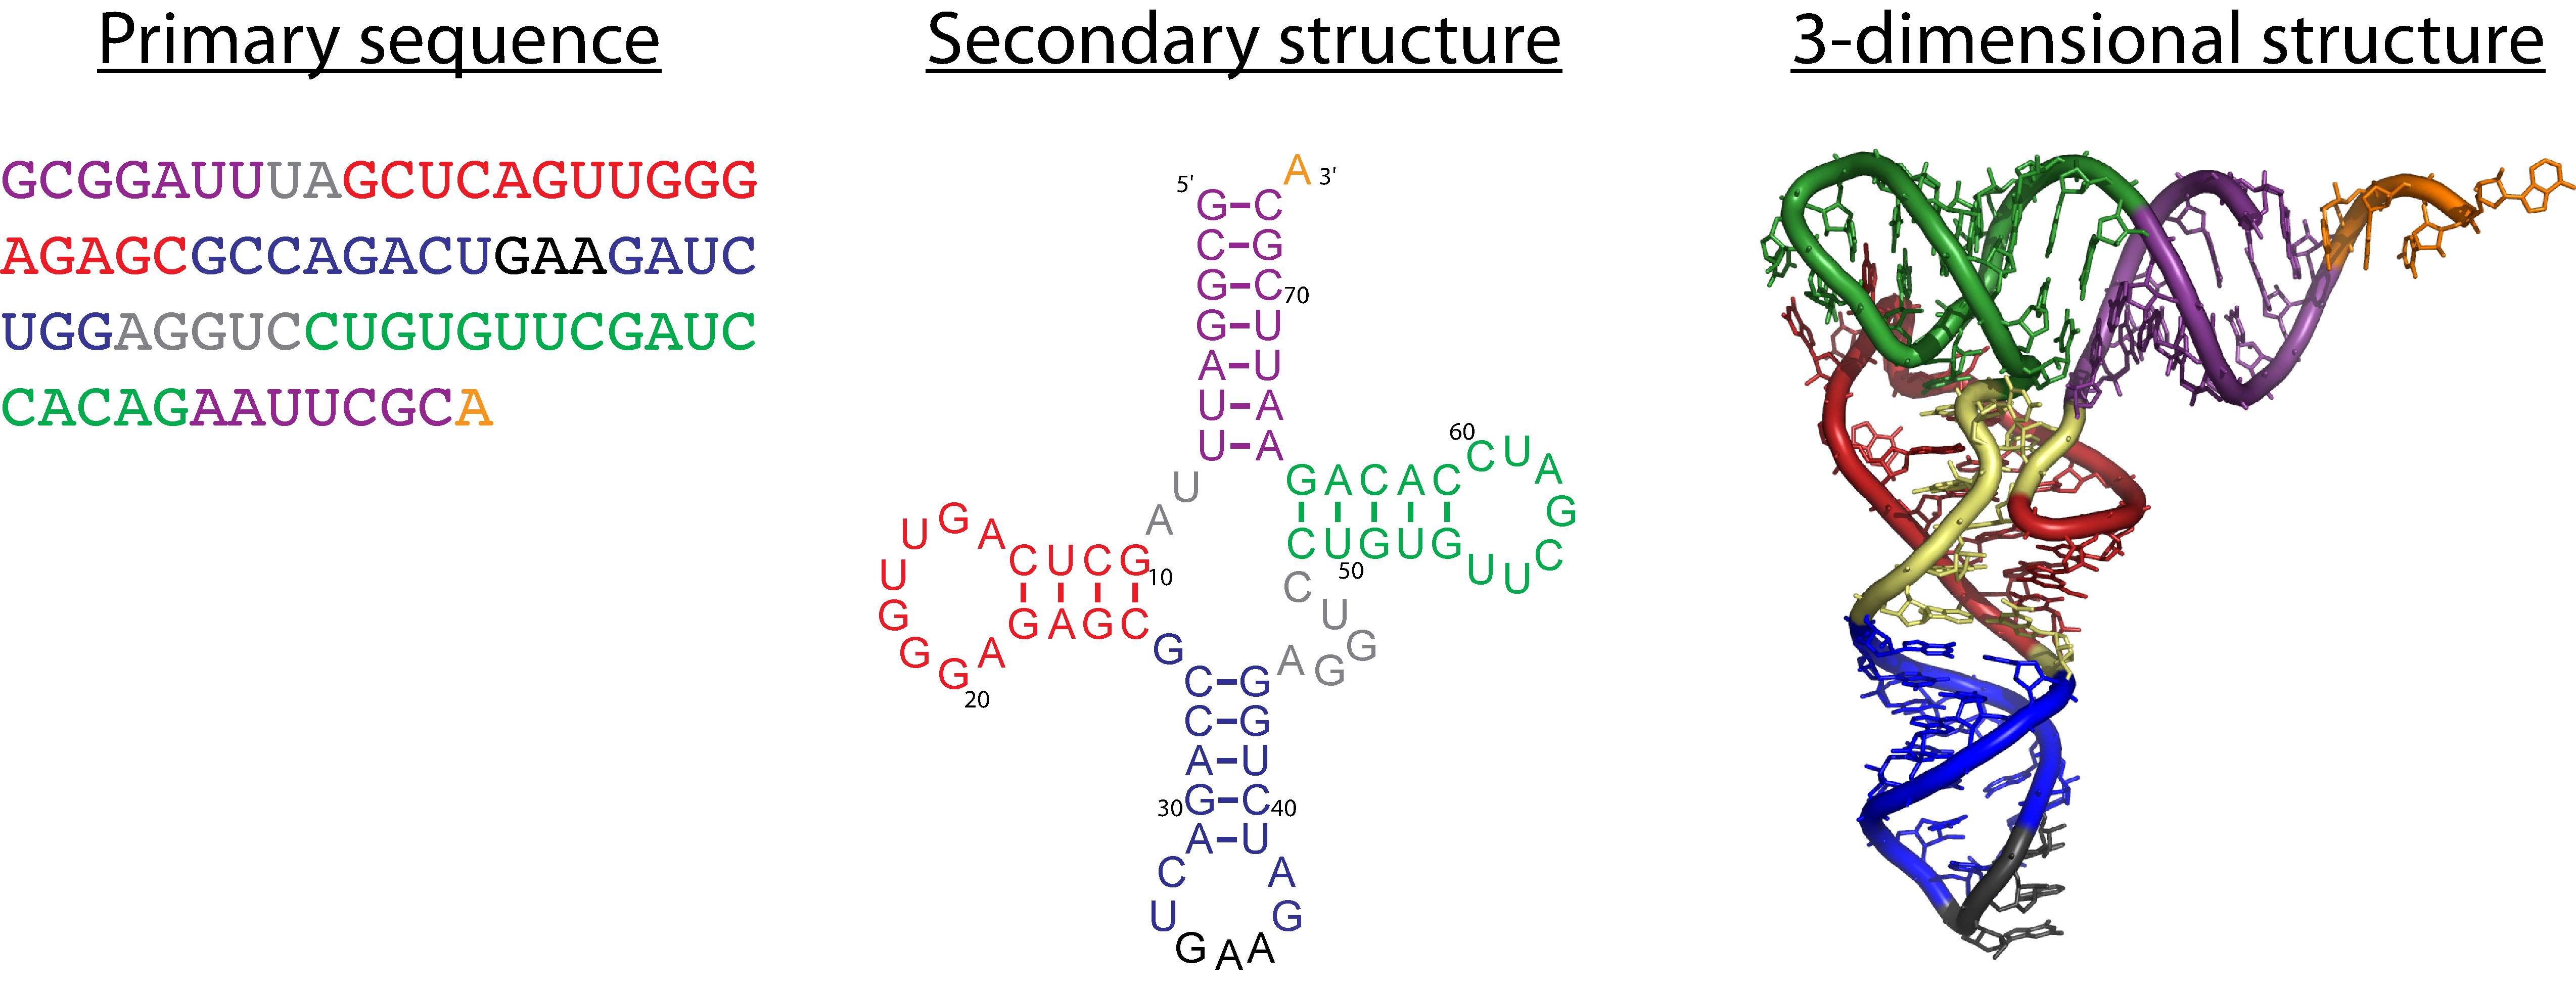
\includegraphics[width=10.5in]{figs/trna-123}
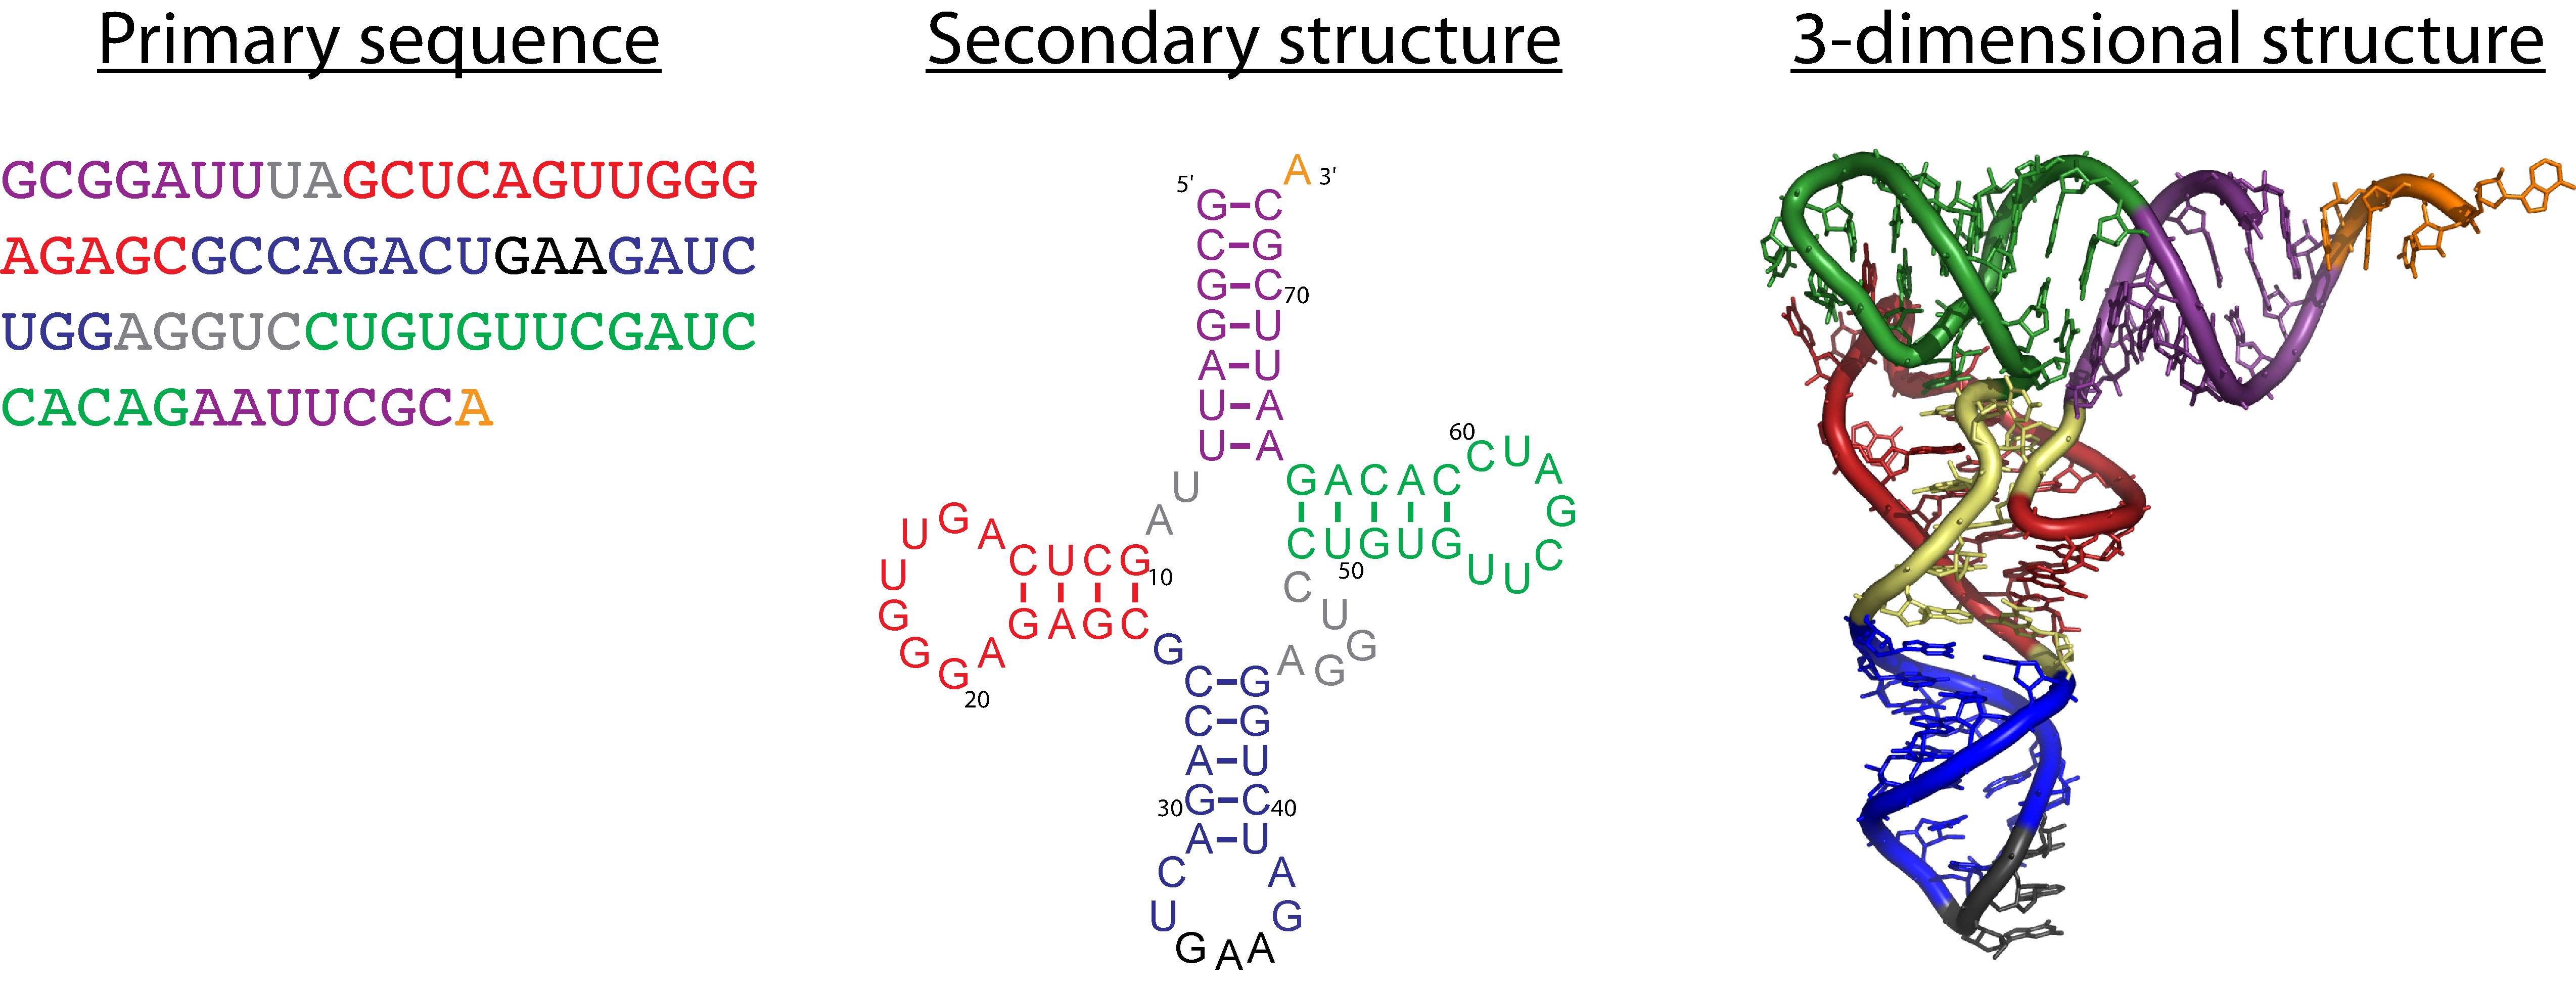
\includegraphics[width=9in]{figs/trna-123}

\end{center}

\vfill

\end{slide}
%%%%%%%%%%%%%%%%%%%%%%%%%%%%%%%%%%%%%%%%%%%%%%%%%%%%%%%%%%%%%%
\begin{slide}
\begin{center}
{\bf Most proteins and RNAs adopt a conserved 3-dimensional 
  structure that is responsible for their function in the cell}

\medskip

Three representations of a transfer RNA:

%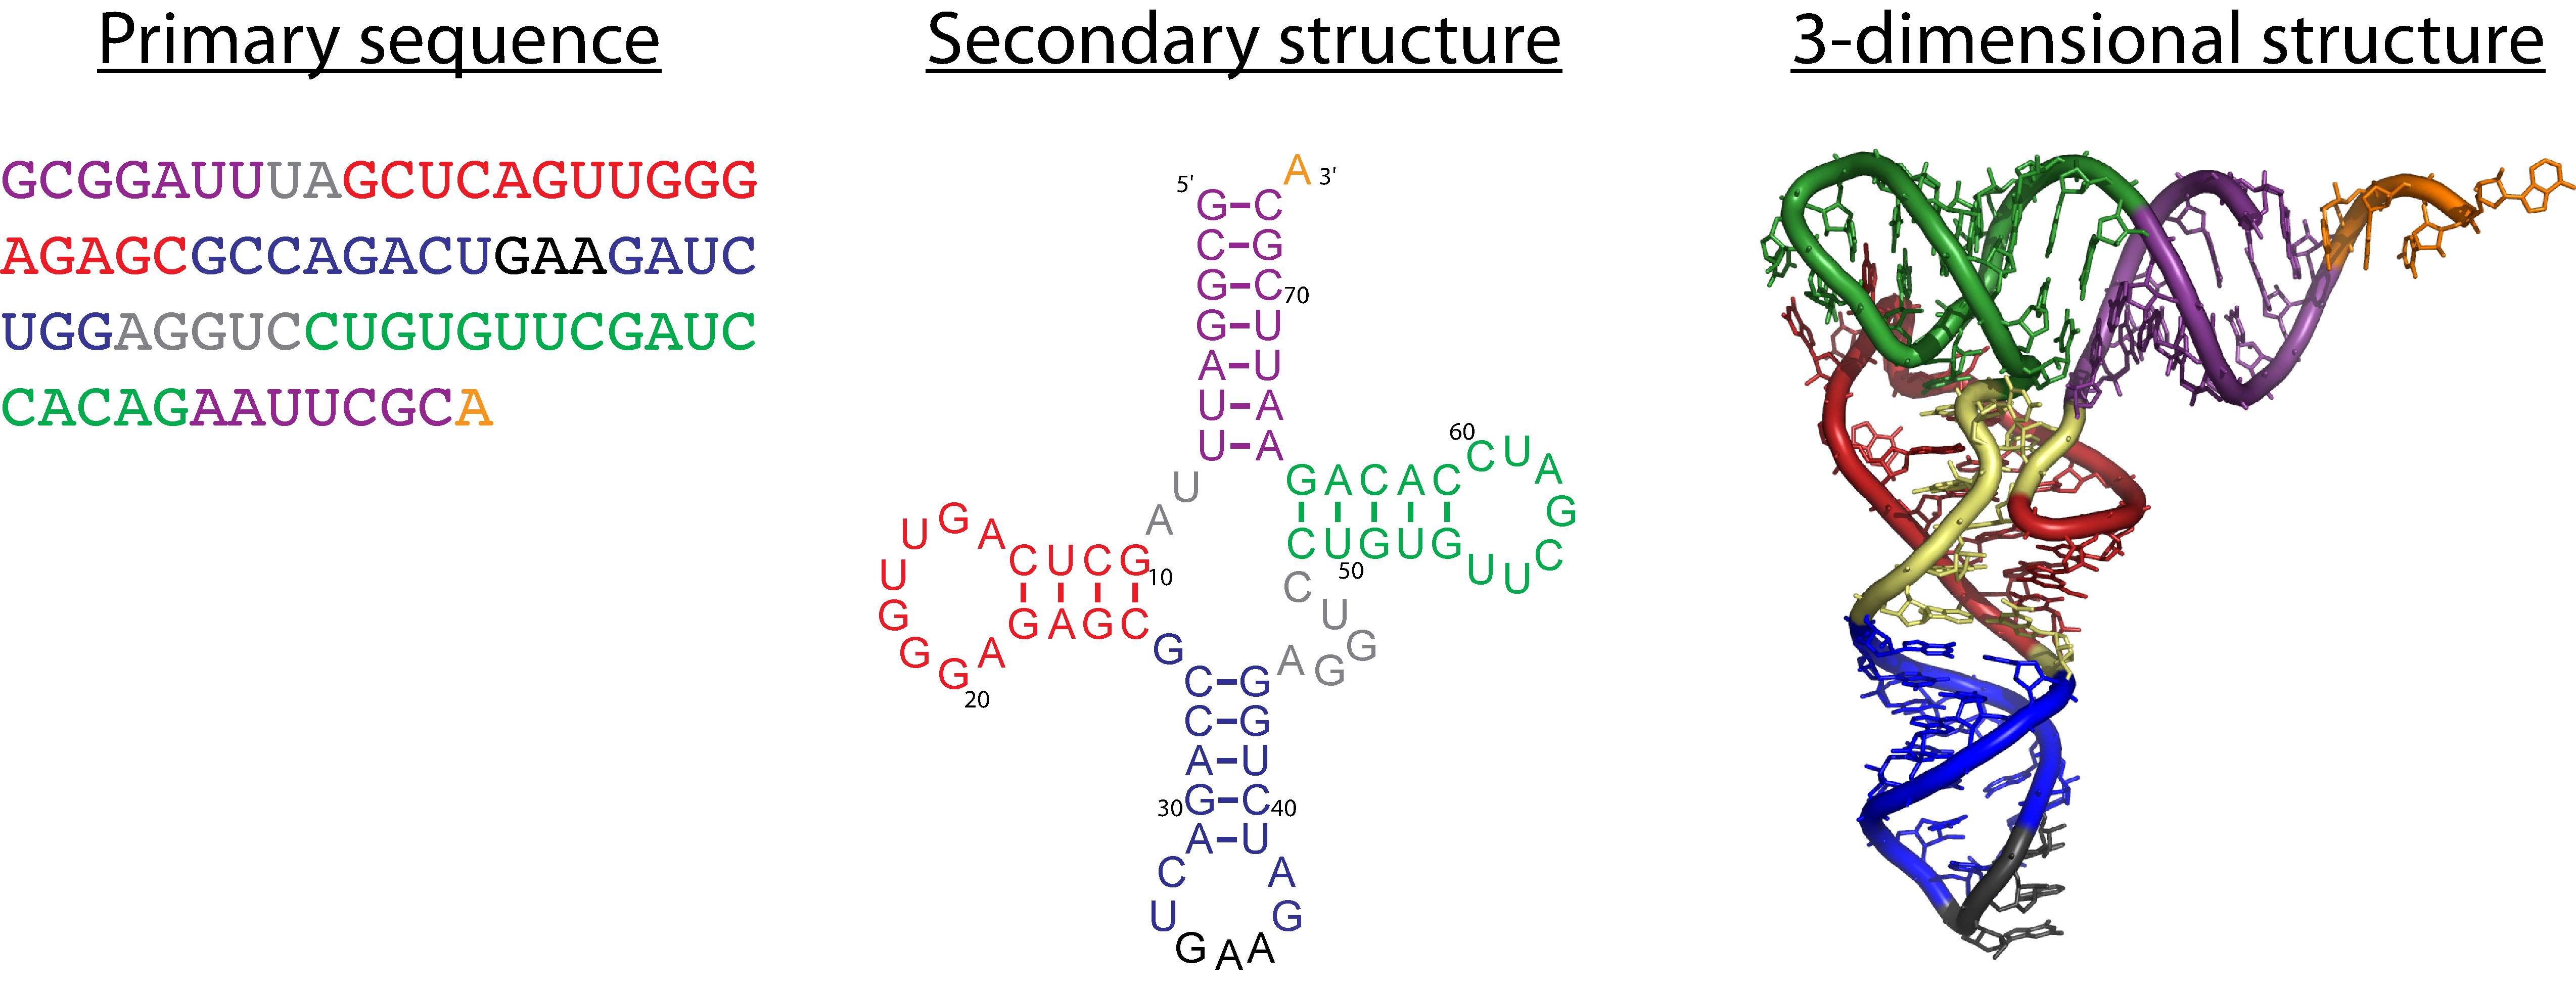
\includegraphics[width=10.5in]{figs/trna-123}
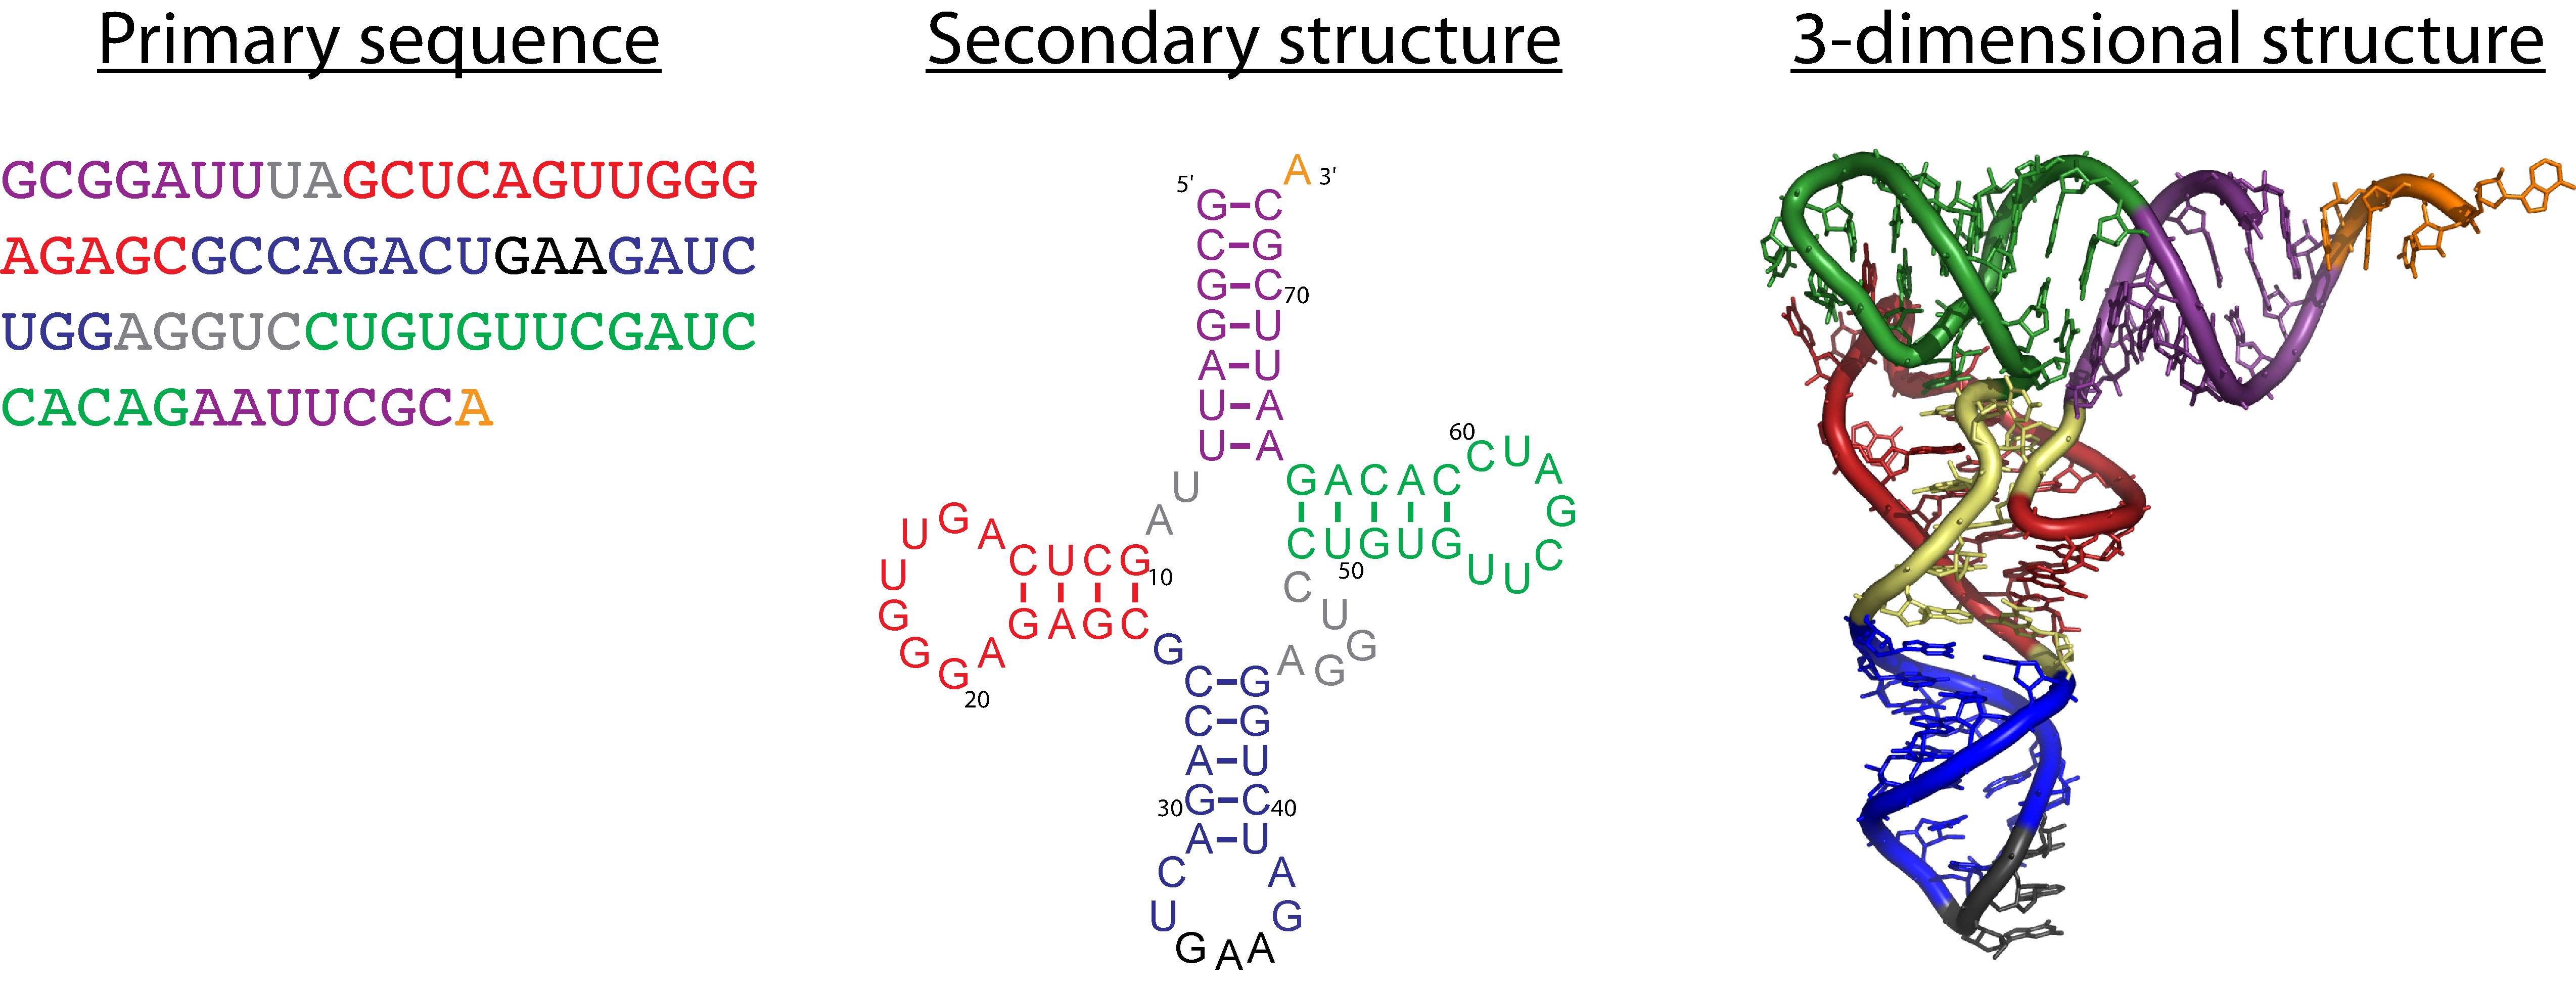
\includegraphics[width=9in]{figs/trna-123}

{\bf BLAST:} given a single sequence, search genomes for similar sequences.

%{\bf Homologous proteins and RNAs conserve \\ both sequence
%and structural features}

{\bf Homologous proteins and RNAs conserve different sequence \\
and structural features to different degrees.}
\end{center}

\vfill

\end{slide}
%%%%%%%%%%%%%%%%%%%%%%%%%%%%%%%%%%%%%%%%%%%%%%%%%%%%%%%%%%%%%
\begin{slide}
\begin{center}
%\textbf{Comparative analysis of sequence families}: \\
\textbf{Sequence conservation provides \\ information for homology searches}
%\emph{Functionally important sequence features are evolutionarily conserved.}
\medskip

%A simple, made-up RNA family:

%Evolution conserves functionally \\ important sequence features.

%Evolution conserves sequence \\ based on its functional importance.

Conservation levels vary across alignment columns.

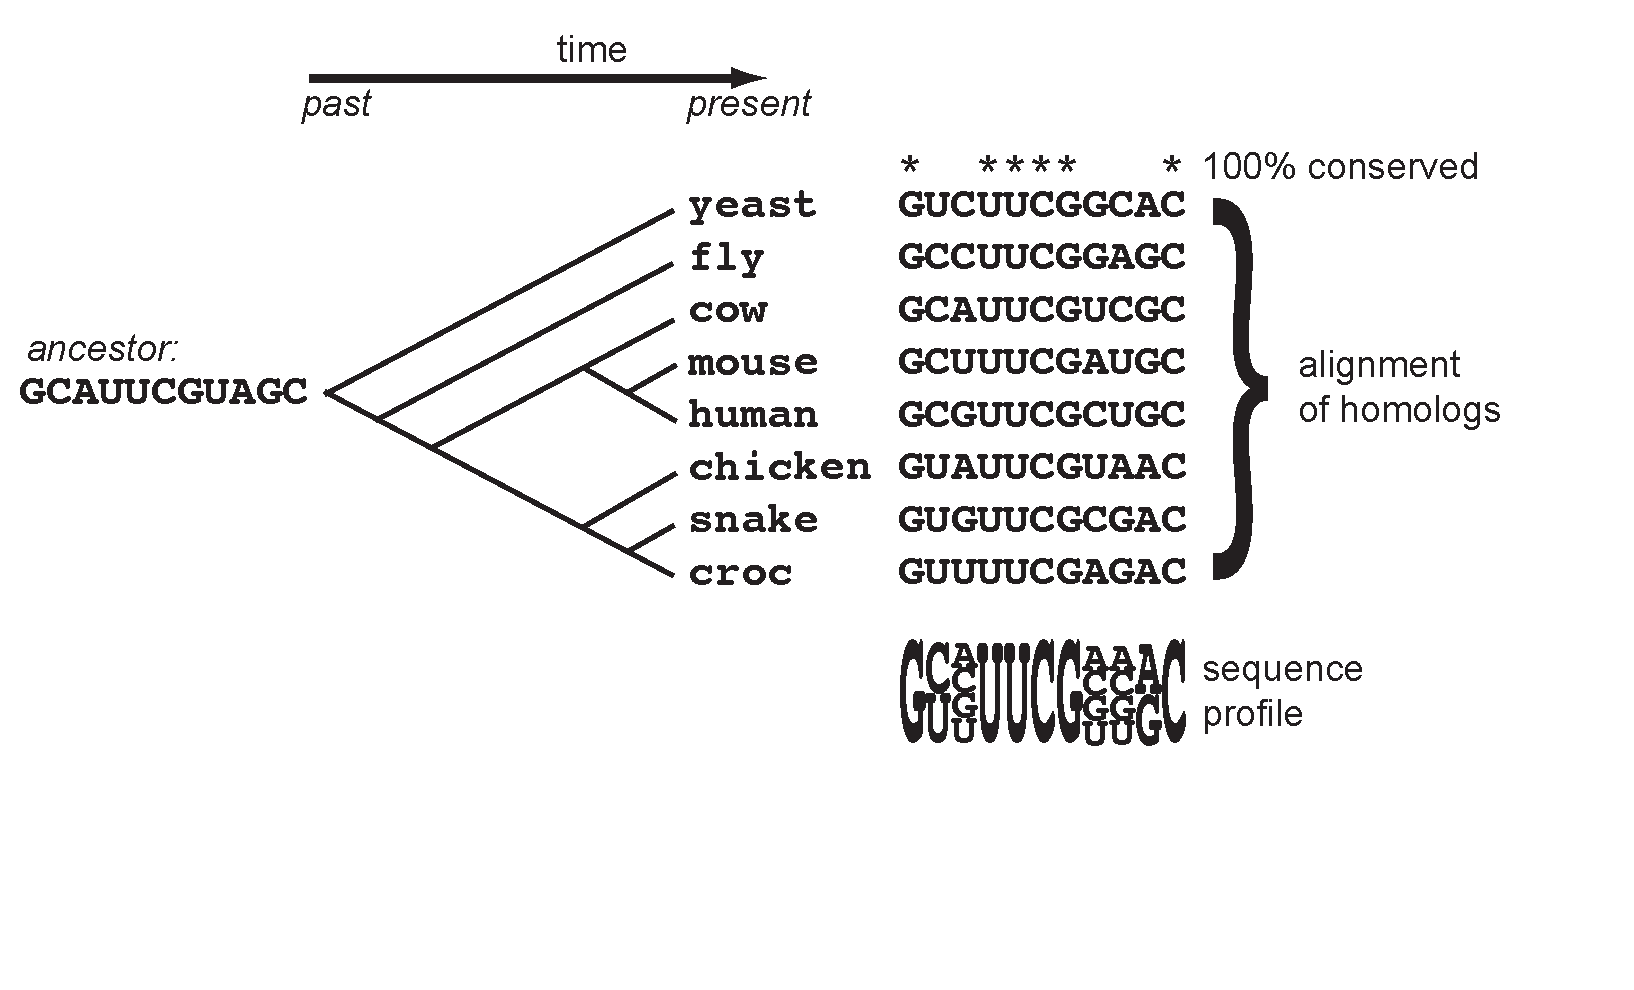
\includegraphics[width=8.625in]{figs/seqstructprofiles-seq1}
\end{center}

\vfill
\end{slide}
%%%%%%%%%%%%%%%%%%%%%%%%%%%%%%%%%%%%%%%%%%%%%%%%%%%%%%%%%%%%%%%%%%%%%%
\begin{slide}
\begin{center}
\textbf{Structure conservation provides additional information}
\medskip

Base-paired positions covary \\ to maintain Watson-Crick complementarity.

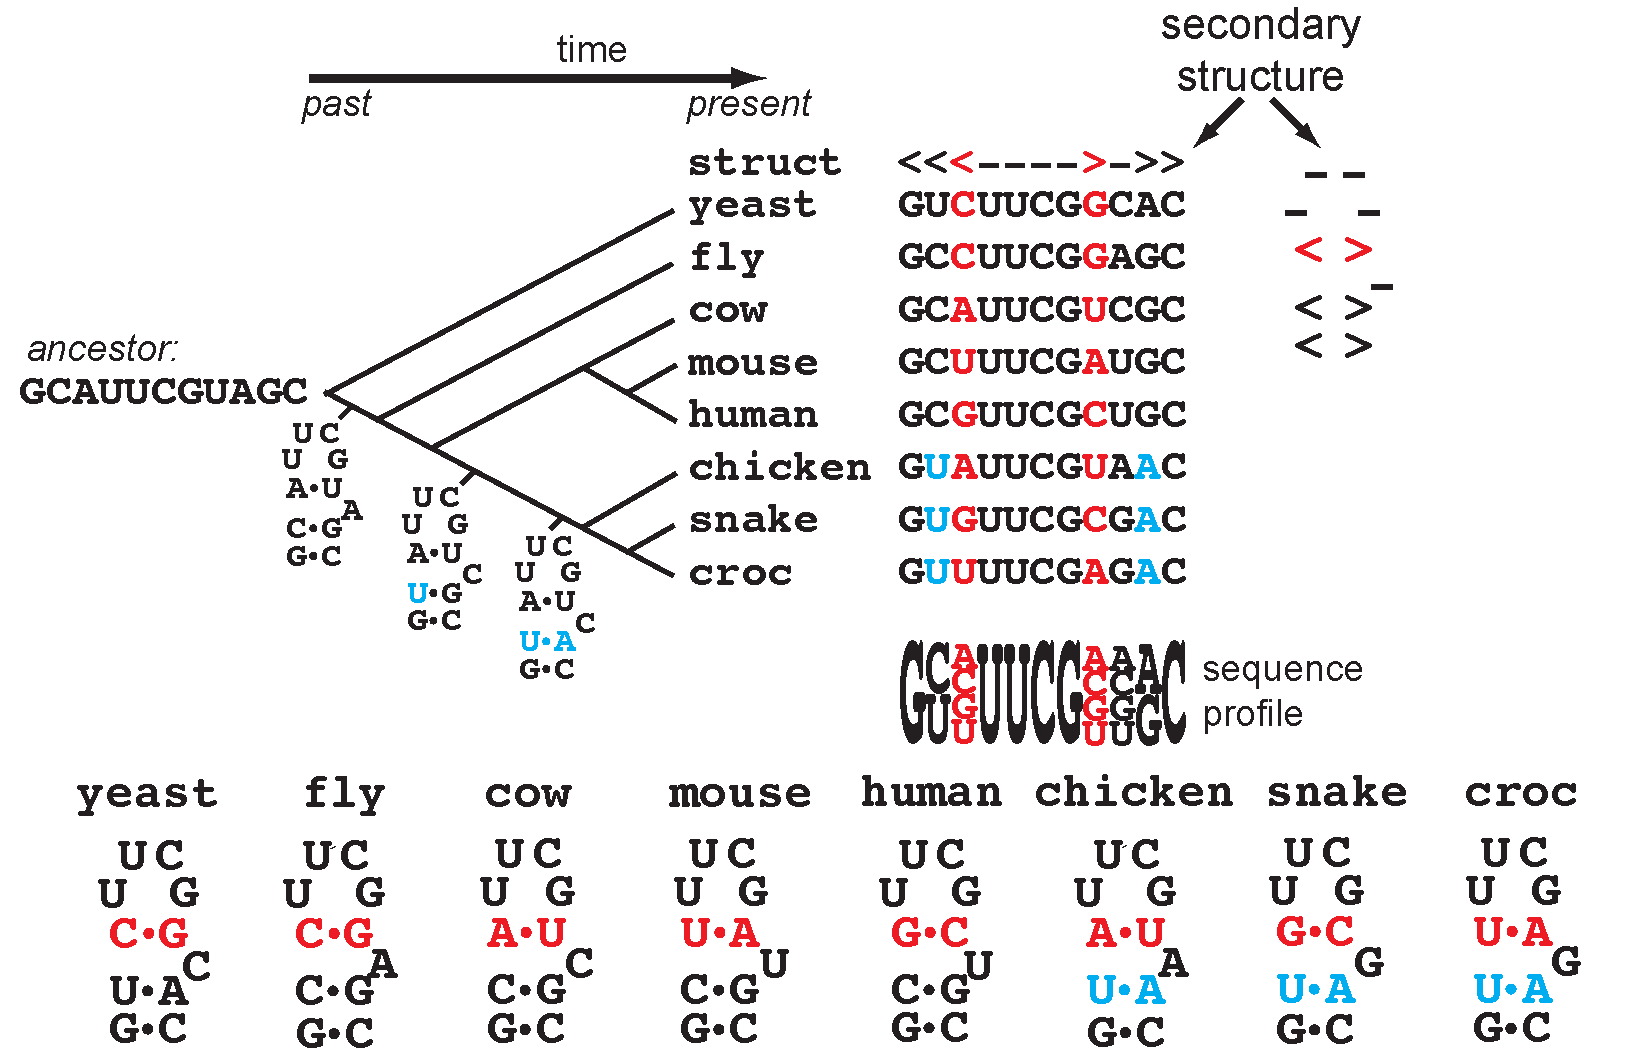
\includegraphics[width=8.625in]{figs/seqstructprofiles-struct2}
\end{center}

\vfill
\end{slide}
%%%%%%%%%%%%%%%%%%%%%%%%%%%%%%%%%%%%%%%%%%%%%%%%%%%%%%%%%%%%%%%%%%%%%%%%%%
\begin{slide}
\begin{center}
\textbf{Levels of sequence and structure conservation in RNA families}
\end{center}
\medskip

\begin{center}
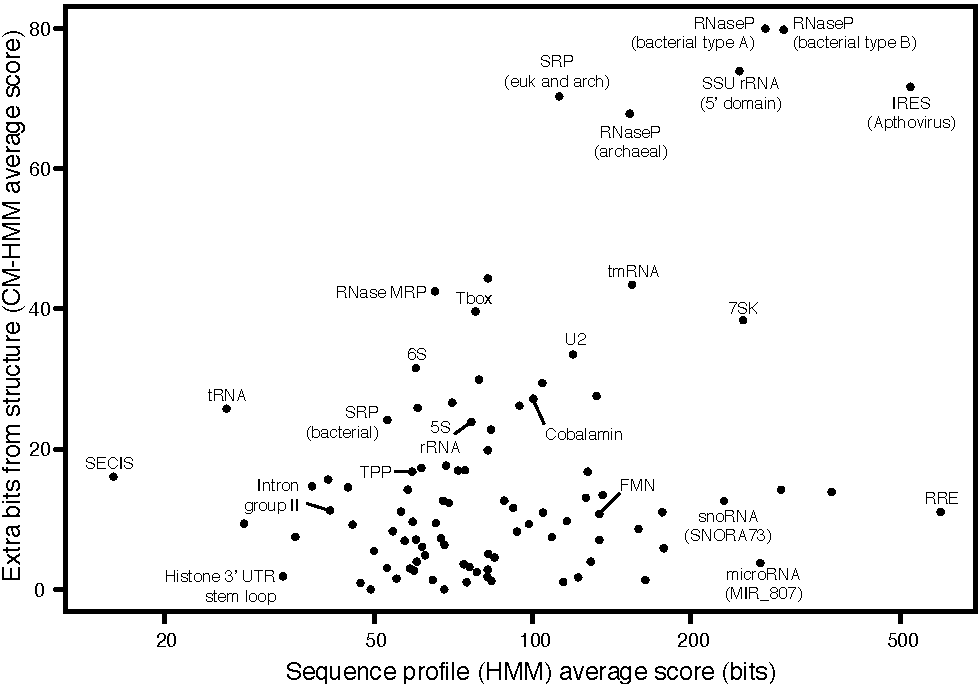
\includegraphics[height=6.5in]{figs/avgscores}
\end{center}

\vfill

\end{slide}
%%%%%%%%%%%%%%%%%%%%%%%%%%%%%%%%%%%%%%%%%%%%%%%%%%%%%%%%%%%%%%%%%%%
\begin{slide}
\begin{center}
%\textbf{profile HMMs and covariance models}
\textbf{Eddy lab software for profile probabilistic models } (since 1994)
\end{center}
\medskip

\begin{center}
\small
\begin{tabular}{r|cc} 
%             &         & sequence \\
%             & sequence& and structure \\
%             & profiles& profiles \\ \hline
             & sequence & sequence and \\
             & profiles & structure profiles \\ \hline
  \\
  models     & profile HMMs     & {\color{red} covariance models (CMs)} \\ 
  \\
  software   & {\sc HMMER}      & {\sc Infernal} \\ 
  \\
  main use   & proteins         & RNAs \\ 
  \\
  database   & {\sc Pfam}       & {\sc Rfam} \\
             & (14831 families) & (2208 families) \\
  \\
%  primary sequence & yes & yes \\
%  \\
%  secondary structure & no & yes \\
%  \\
%  algorithms & Viterbi, Forward & CYK, Inside \\
%%             & Forward & Inside \\
%             &         & \\
%  complexity & $O(LN)$ & $O(LN^{2} log N)$ \\
%  \\
  performance& faster but    & slower but    \\
  for RNAs   & less accurate & more accurate \\
\end{tabular}

%\hspace{1.2in}\includegraphics[height=2in]{figs/hmmer_logo}\hspace{1.05in}\includegraphics[height=2.6in]{figs/infernal_logo}
\hspace{1.2in}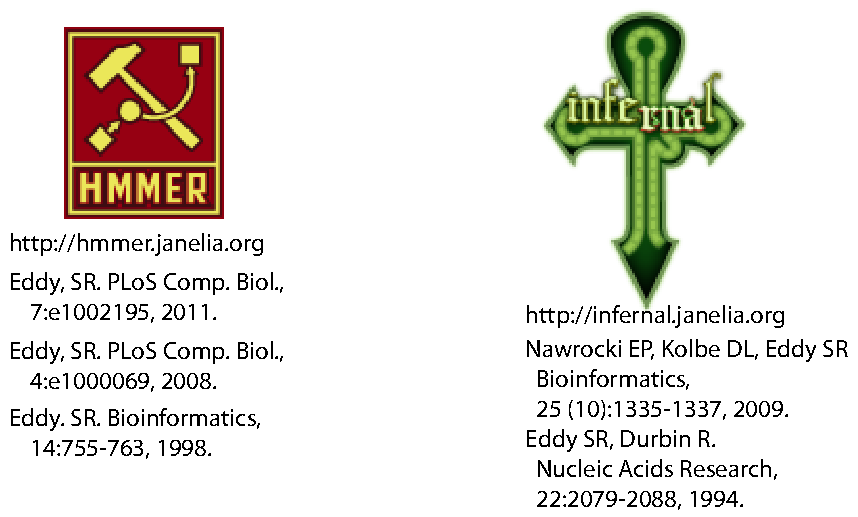
\includegraphics[height=2.7in]{figs/hmmer-infernal-refs}

\end{center}

\vfill

\end{slide}
%%%%%%%%%%%%%%%%%%%%%%%%%%%%%%%%%%%%%%%%%%%%%%%%%%%%%%%%%%%%%%%
%%%%%%%%%%%%%%%%%%%%%%%%%%%%%%%%%%%%%%%%%%%%%%%%%%%%%%%%%%%%%%%%%%%%
\begin{slide}
\begin{center}
%\textbf{profile HMMs and covariance models}
\textbf{Profile HMMs: sequence family models built from alignments}
\end{center}

\center{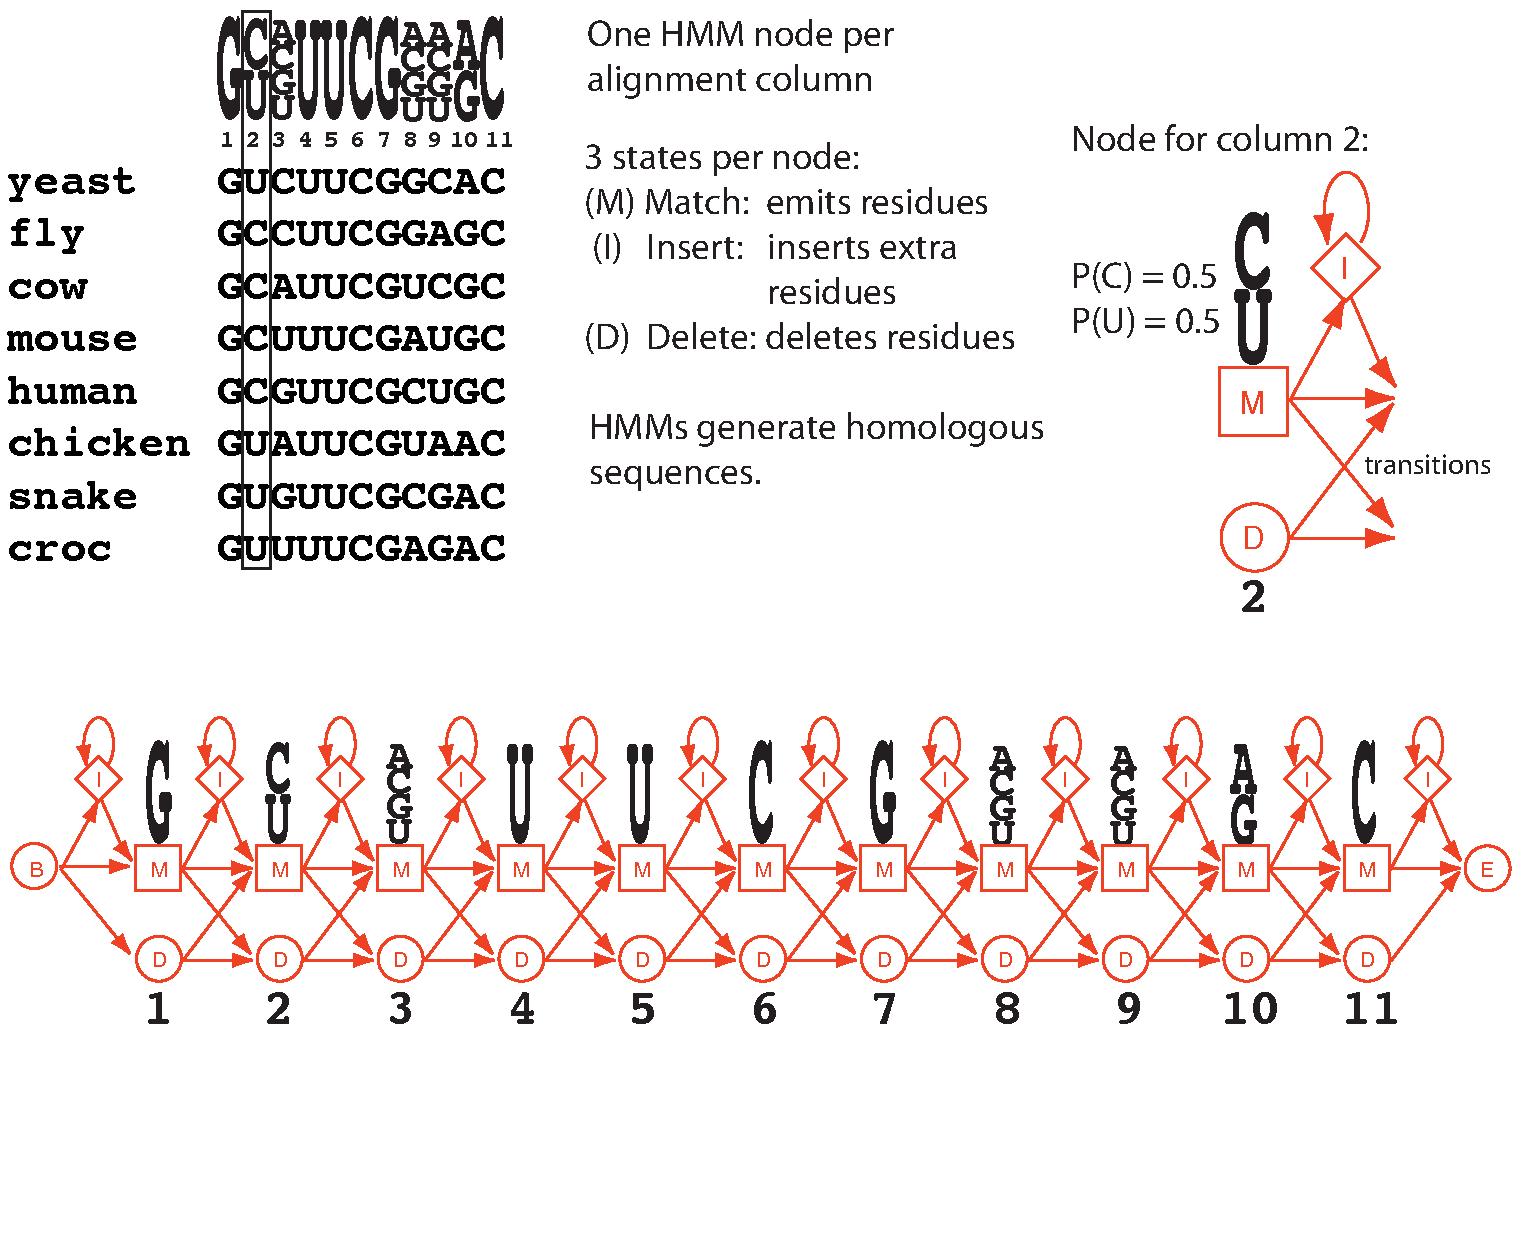
\includegraphics[height=6.625in]{figs/hmm}}

%An HMM generates ``homologous'' sequences.

\end{slide}
%%%%%%%%%%%%%%%%%%%%%%%%%%%%%%%%%%%%%%%%%%%%%%%%%%%%%%%%%%%%%%%
\begin{slide}
\begin{center}
%\textbf{profile HMMs and covariance models}
\textbf{Profile HMMs: sequence family models built from alignments}
\end{center}

\center{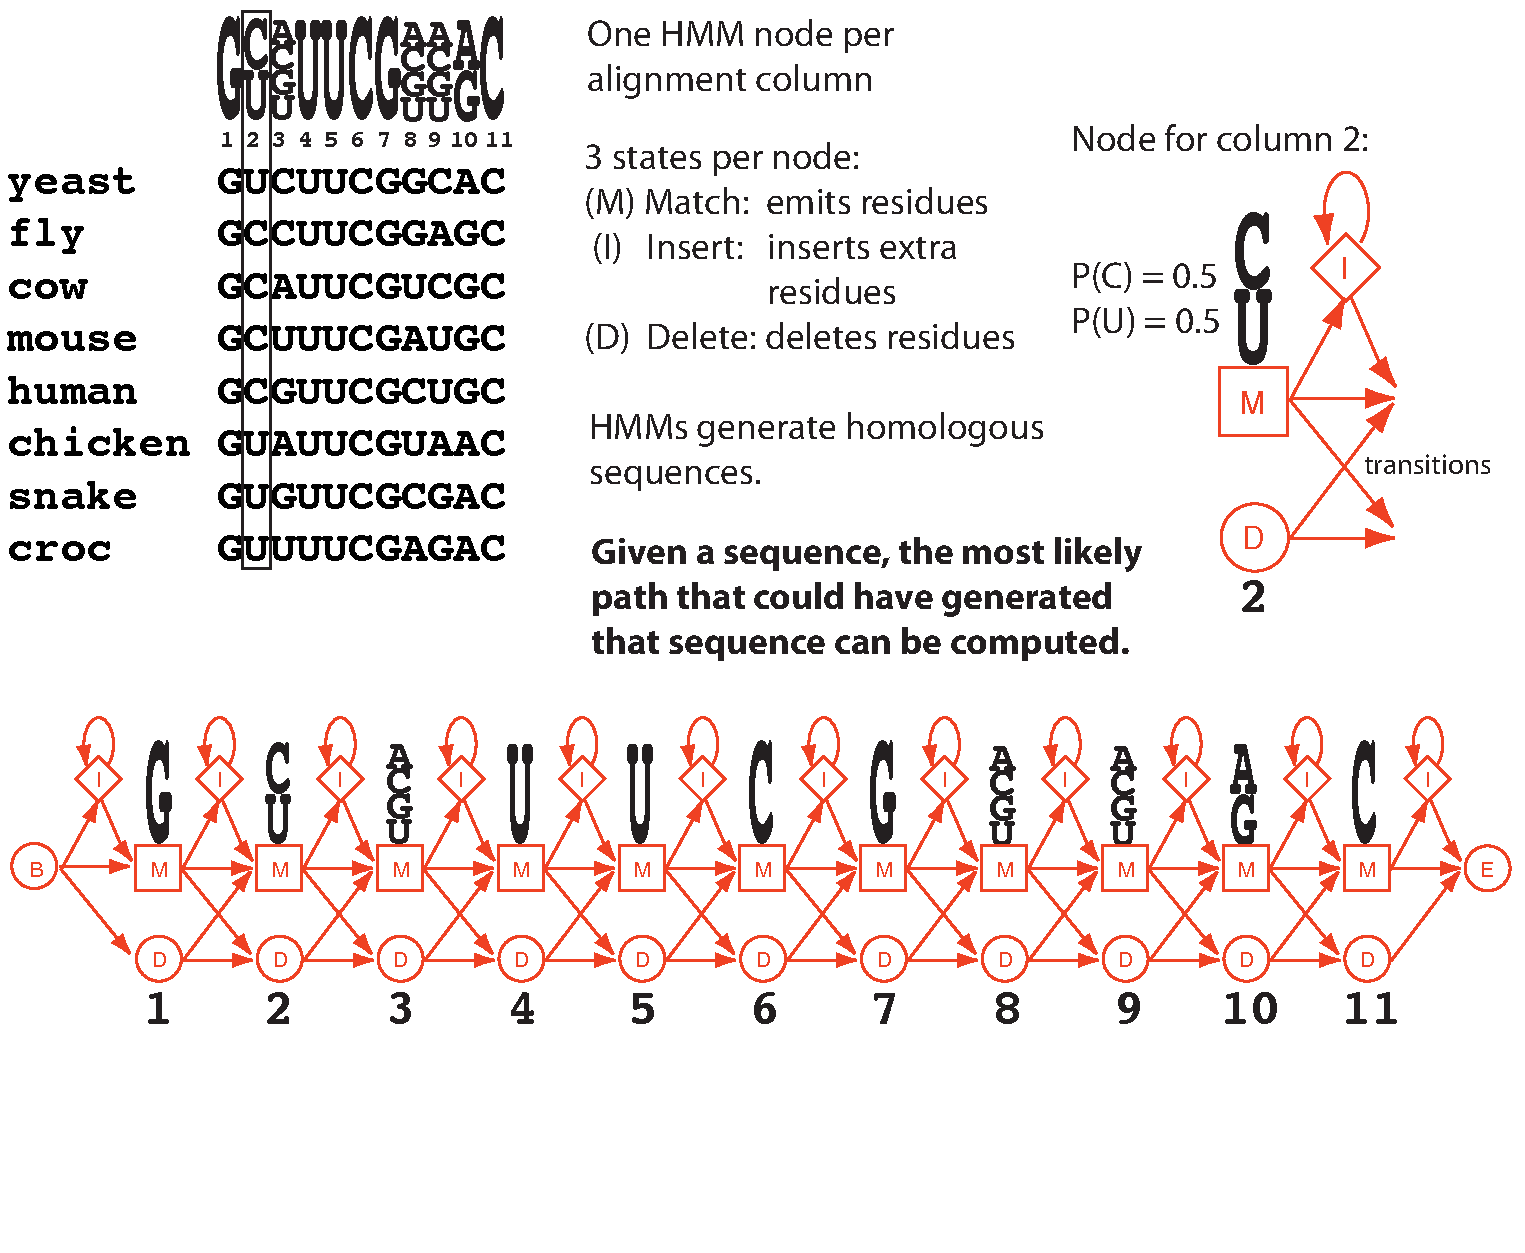
\includegraphics[height=6.625in]{figs/hmm-given}}
\end{slide}
%%%%%%%%%%%%%%%%%%%%%%%%%%%%%%%%%%%%%%%%%%%%%%%%%%%%%%%%%%%%%%%
\begin{slide}
\begin{center}
%\textbf{profile HMMs and covariance models}
\textbf{Profile HMMs: sequence family models built from alignments}
\end{center}

\center{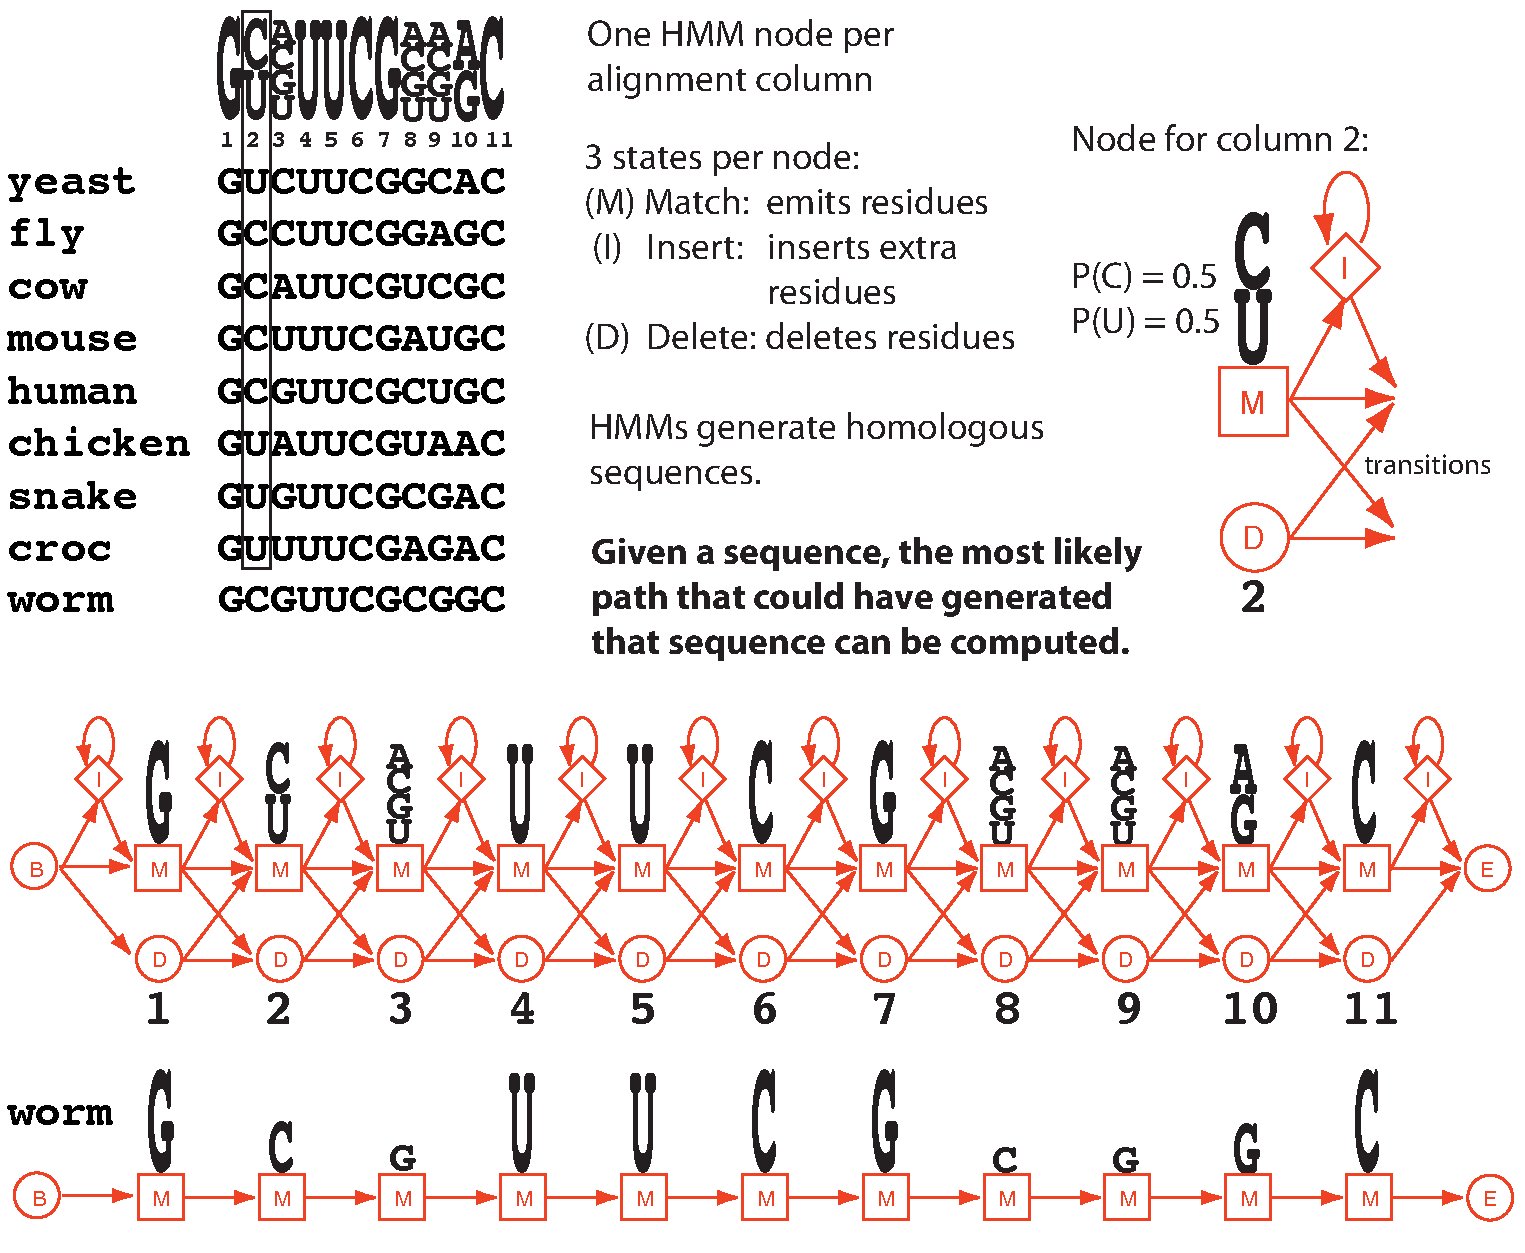
\includegraphics[height=6.625in]{figs/hmm-worm}}
\end{slide}
%%%%%%%%%%%%%%%%%%%%%%%%%%%%%%%%%%%%%%%%%%%%%%%%%%%%%%%%%%%
\begin{slide}
\begin{center}
%\textbf{profile HMMs and covariance models}
\textbf{Profile HMMs: sequence family models built from alignments}
\end{center}

\center{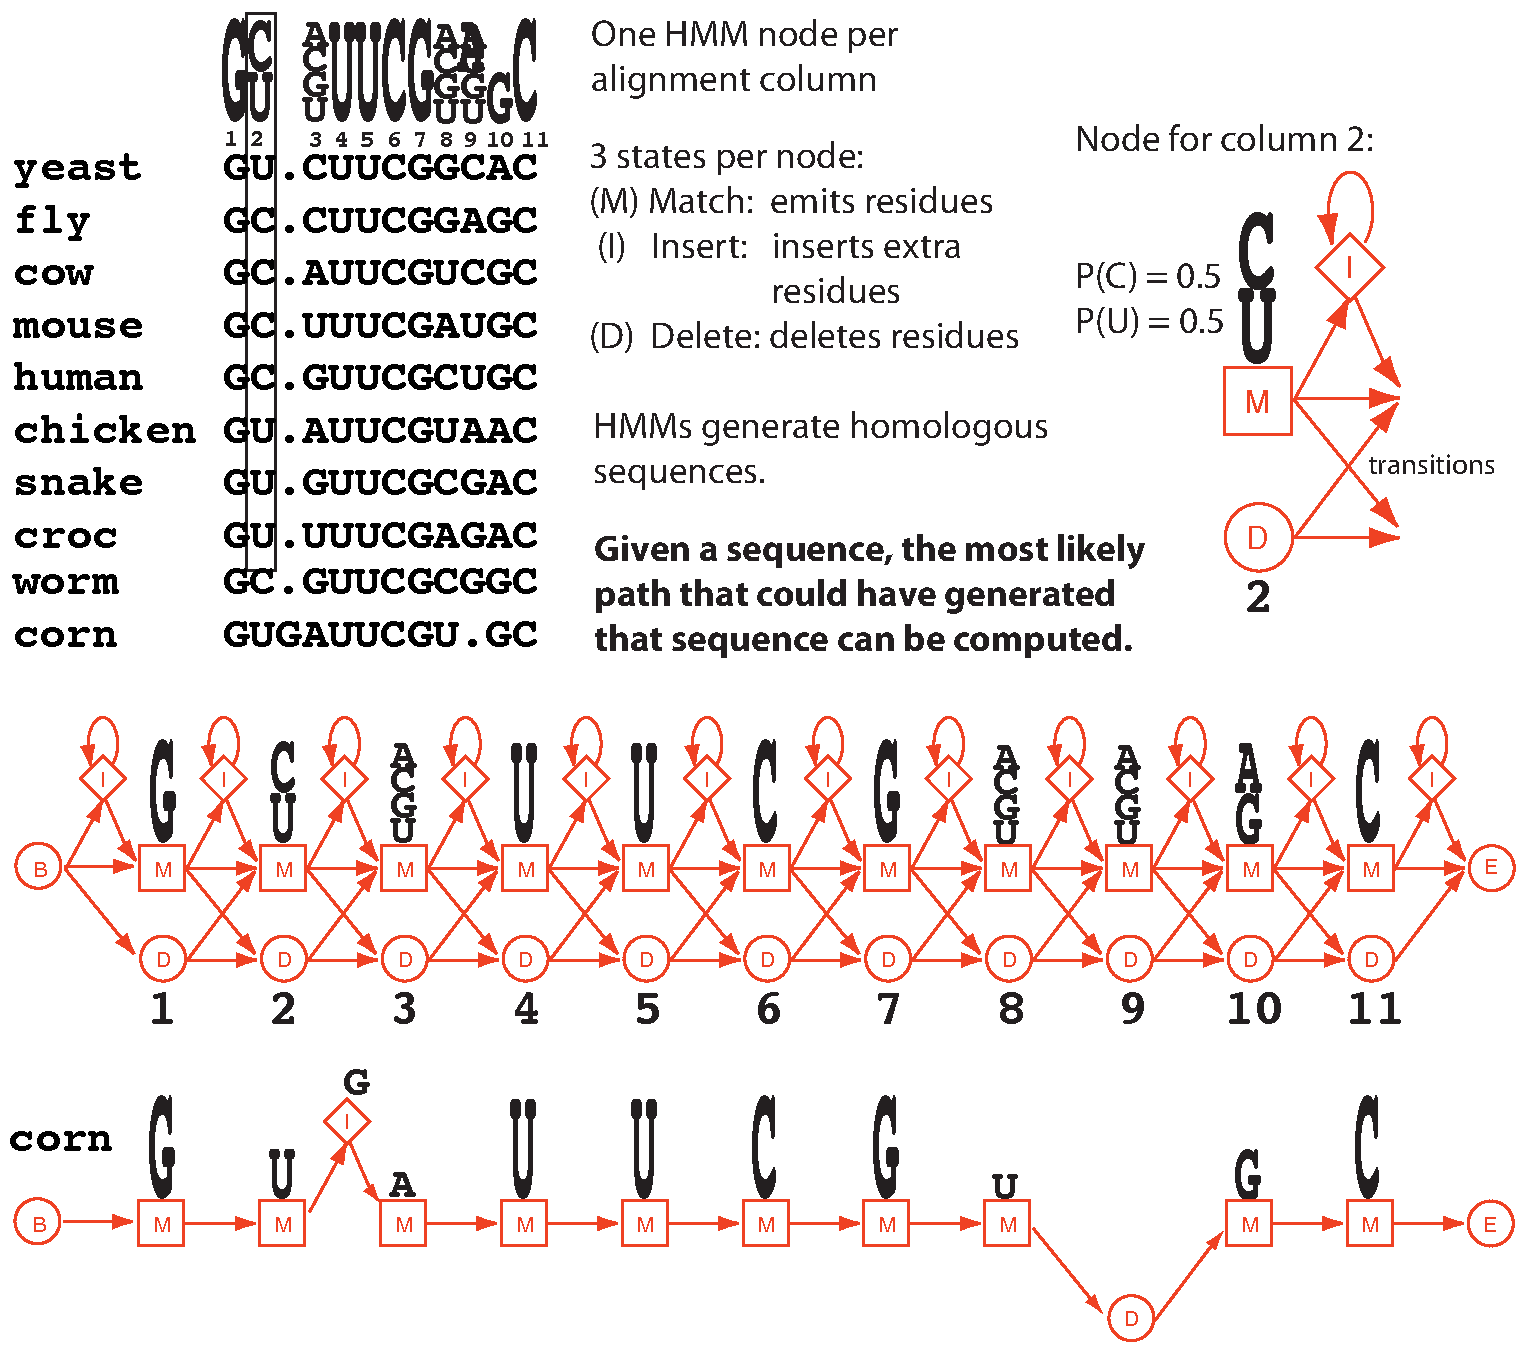
\includegraphics[height=6.625in]{figs/hmm-corn}}
\end{slide}
%%%%%%%%%%%%%%%%%%%%%%%%%%%%%%%%%%%%%%%%%%%%%%%%%%%%%%%%%%%%%%%
\begin{slide}
\begin{center}
%\textbf{profile HMMs and covariance models}
\textbf{Covariance models (CMs) are built \\ from structure-annotated alignments}
\end{center}

\center{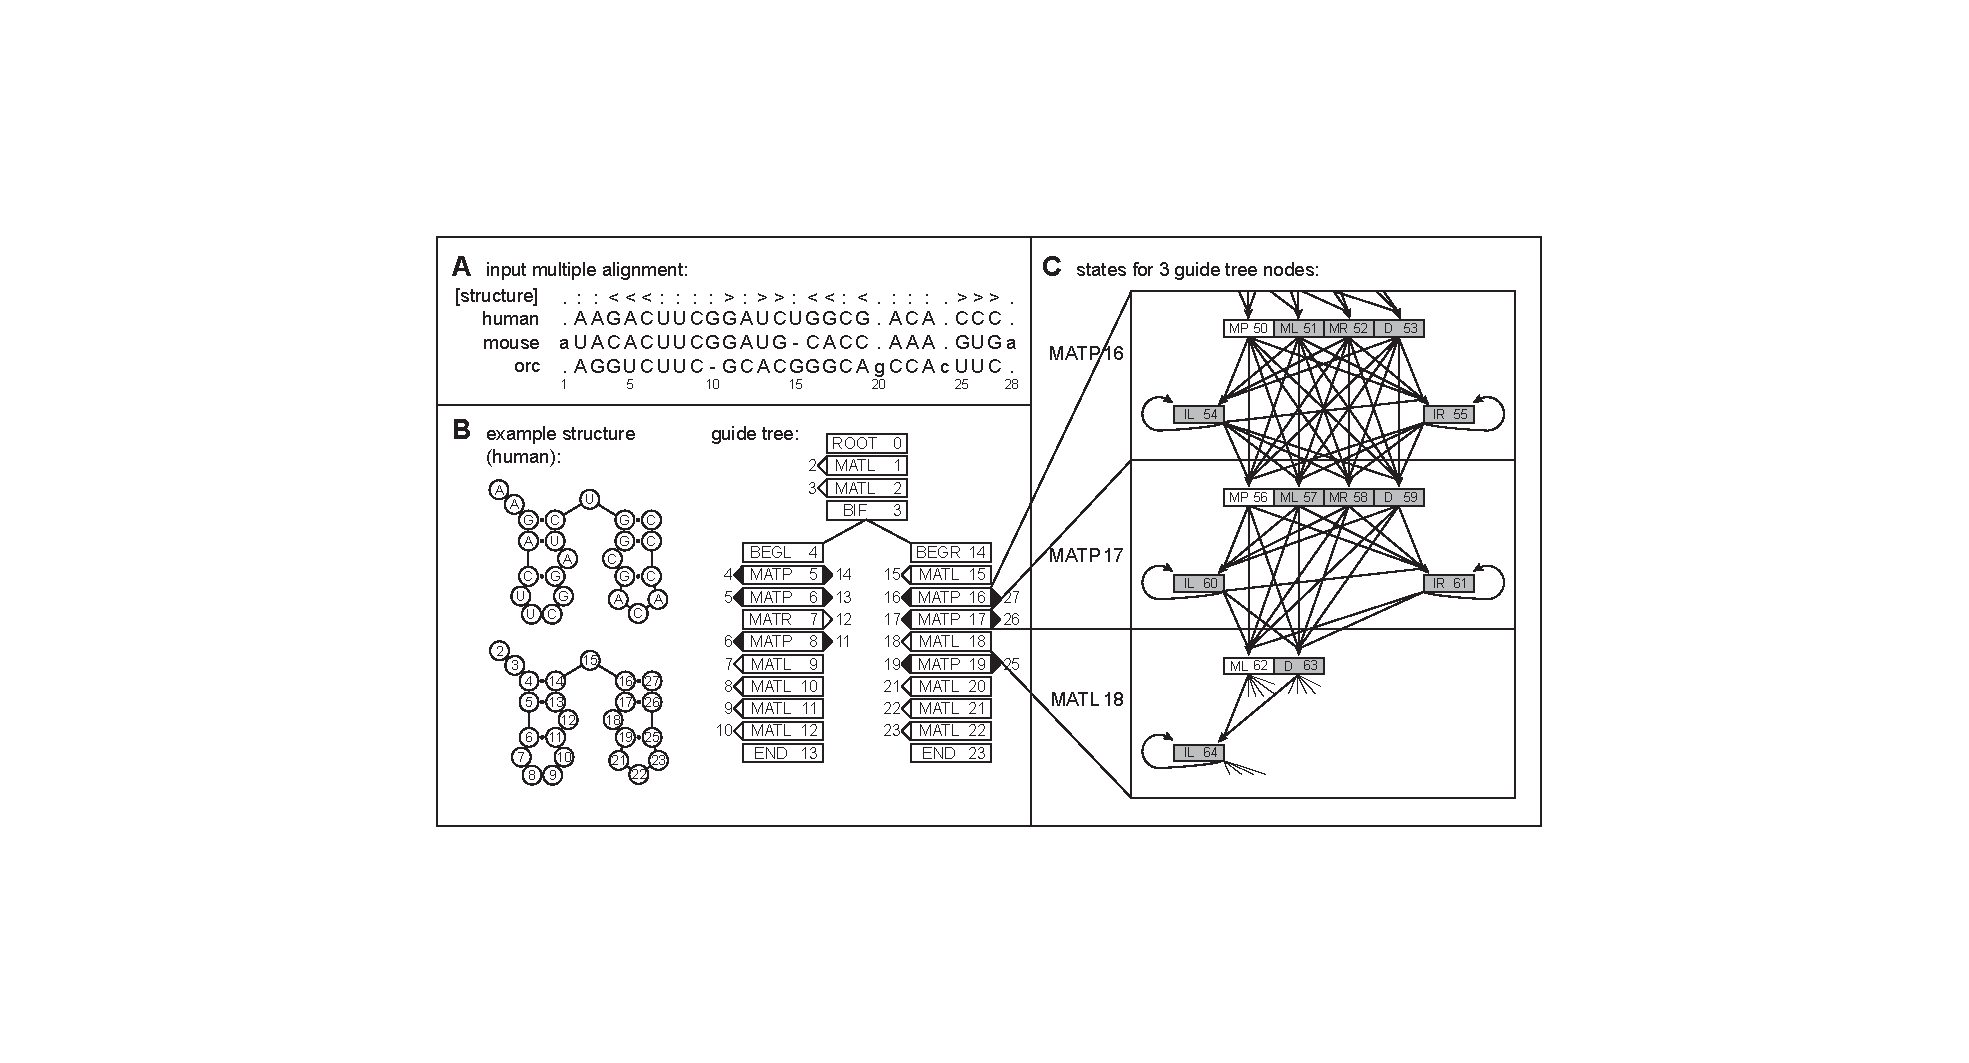
\includegraphics[width=7in]{figs/cmintro_bandcyk}}

\center{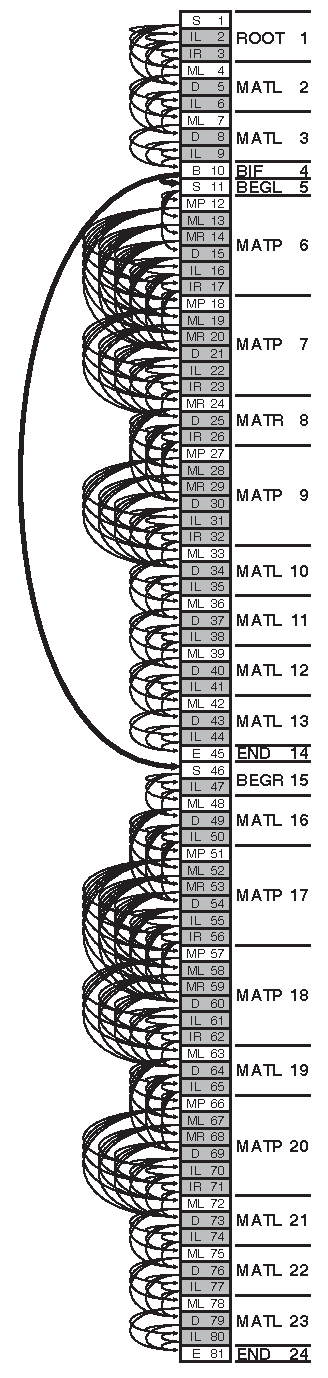
\includegraphics[width=2in,angle=270]{figs/cm-graph-small}}

\vfill

\end{slide}
%%%%%%%%%%%%%%%%%%%%%%%%%%%%%%%%%%%%%%%%%%%%%%%%%%%%%%%%%%%%%%%%%%
\begin{slide}
\begin{center}
\textbf{Is the added complexity worth it? \\
  RMARK: a challenging \underline{internal} RNA homology search \\
  benchmark for use during Infernal development}
\end{center}
\medskip
\begin{minipage}{7in}
\small
\begin{itemize}
\item
  RMARK construction - for each of the 1446 Rfam 10 seed alignments:
  \begin{itemize}
%  \item
%    remove sequences $<$ 70\% average family length
  \item 
    cluster sequences by sequence identity \\ given the alignment
  \item 
    look for a \textcolor{blue}{training} cluster and
    \textcolor{red}{testing} cluster such that: 
    \begin{itemize}
    \item
      no \textcolor{blue}{training}/\textcolor{red}{test} sequence pair is $>$ 60\% identical
    \item
      at least five sequences are in the \textcolor{blue}{training} set
    \end{itemize}
  \item
    filter \textcolor{red}{test} set so no two test seqs $>$ 70\% identical 
  \item
    %51 families qualify, with 450 \textcolor{red}{test} sequences
    106 families qualify, with 780 test sequences
  \item
    %\textcolor{red}{test} seqs are embedded in a 1 Mb pseudo-genome (25\% A,C,G,U)
    test seqs are embedded in a 10 Mb pseudo-genome of ``realistic'' base composition
%  \item
%    %    \textsc{BLAST}: family-pairwise search, each \textcolor{blue}{training} seq is used
%        \textsc{BLAST}: family-pairwise search, each \\ training sequence is used
%    as a separate query
%  \item
%    %\textsc{Infernal}: build 1 CM per family from \textcolor{blue}{training} set
%    \textsc{Infernal}: build 1 CM per family from \\ training alignment 
  \end{itemize}
\end{itemize}
\vspace{1.5in}
\end{minipage}
\hspace{0.1in}
\begin{minipage}{3.5in}
  Example: 
\vspace{0.2in}

\begin{center}
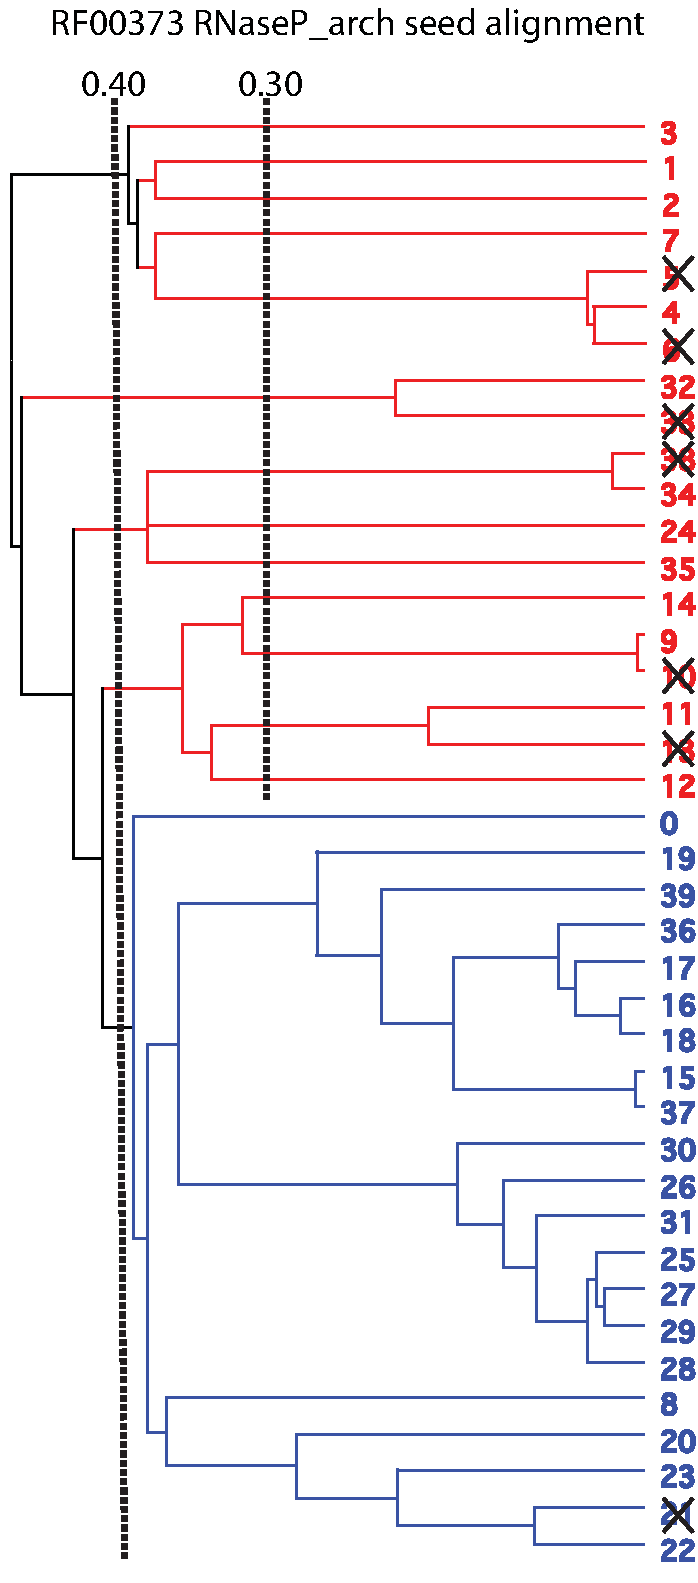
\includegraphics[height=5.5in]{figs/u8-RF00373-tree}

\end{center}
\end{minipage}
\end{slide}
%%%%%%%%%%%%%%%%%%%%%%%%%%%%%%%%%%%%%%%%%%%%%%%%%%%%%%%%%%%%%%%%%%%%%%
\begin{slide}
\begin{center}

\textbf{Infernal outperforms primary-sequence based methods on our
  benchmark (and others\footnote{Freyhult EK, Bollback JP, Gardner
    PP. Genome Res. 2007 17: 117-125.}, not shown)}

\end{center}
\medskip

\center{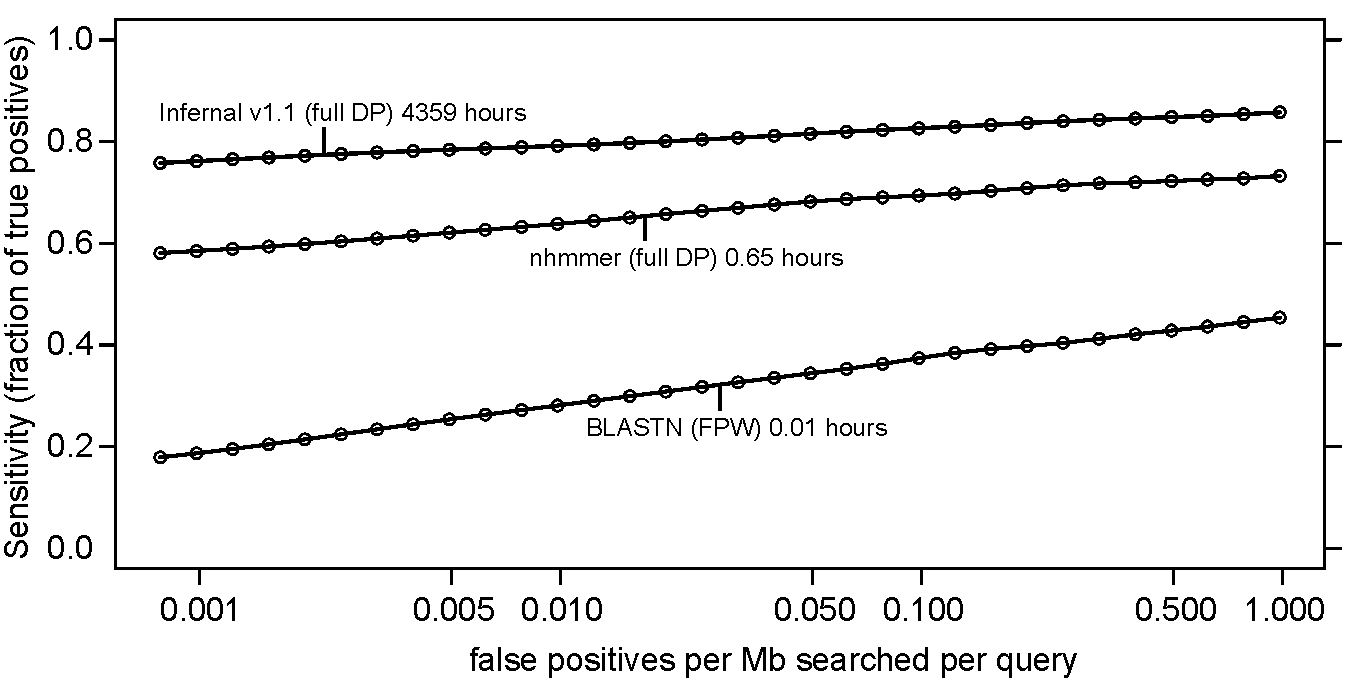
\includegraphics[width=10in]{figs/roc1-jsm}}

\vfill 
\end{slide}
%%%%%%%%%%%%%%%%%%%%%%%%%%%%%%%%%%%%%%%%%%%%%%%%%%%%%%%%%%%%%%%%%%%%%%
\begin{slide}
\begin{center}

\textbf{Over the last several years we've accelerated \\ HMMER and
  Infernal by several orders of magnitude}
\end{center}
\medskip

\center{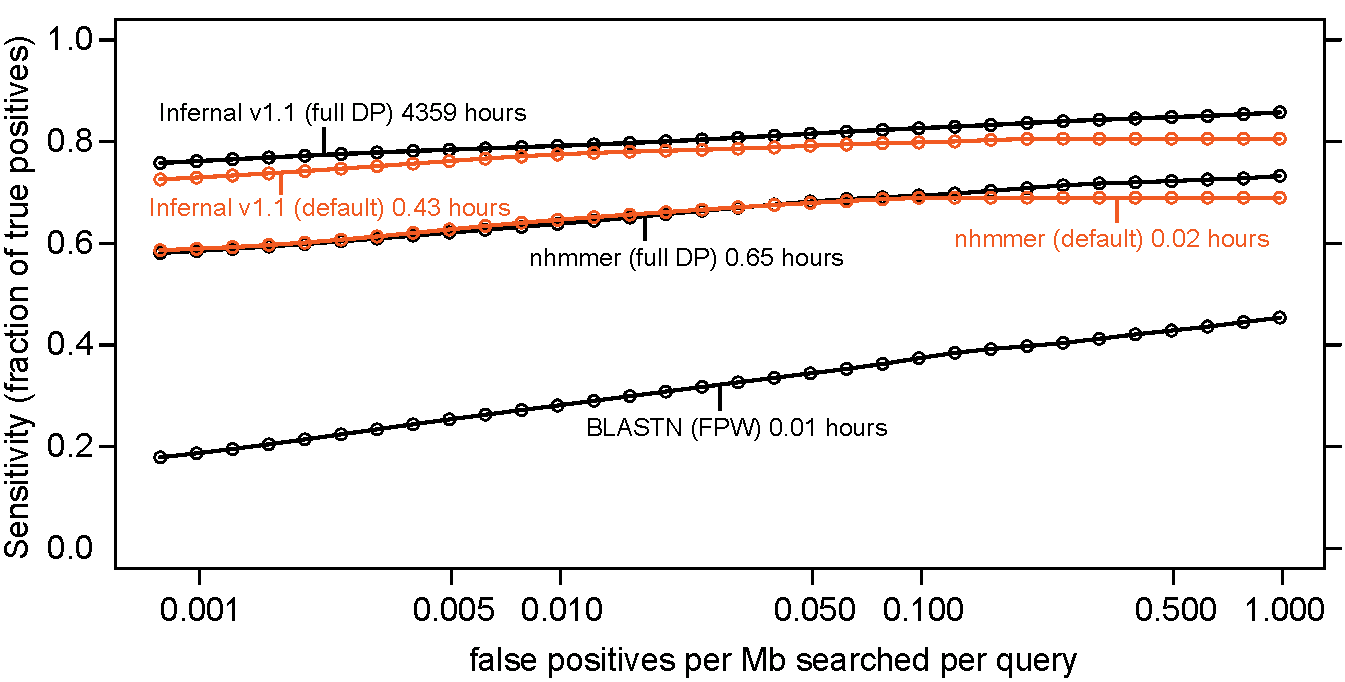
\includegraphics[width=10in]{figs/roc2-jsm}}

\vfill 
\end{slide}
%%%%%%%%%%%%%%%%%%%%%%%%%%%%%%%%%%%%%%%%%%%%%%%%%%%%%%%%%%%%%%%%%%%%%%
\begin{slide}
\begin{center}
\textbf{MSV filter for faster profile HMM searches}
\end{center}

\medskip

\begin{itemize}

\small
\item MSV (Multiple Segment Viterbi) algorithm, which disallows inserts
  and deletes, can be computed using 16-fold vector parallelism with
  low-precision (8-bit) scores\footnote{Eddy SR. PLoS Comp. Biol., 7:e1002195, 2011}.

\end{itemize}

\center{\includegraphics[height=4in]{figs/msv-trunc}}

\vfill 
\end{slide}
%%%%%%%%%%%%%%%%%%%%%%%%%%%%%%%%%%%%%%%%%%%%%%%%%%%%%%%%%%%%%%%%%%%%%%
\begin{slide}
\begin{center}
\textbf{HMM filters and constrained DP for faster CM searches}
\end{center}

\medskip

\small
\begin{itemize}
\item Infernal uses HMMER's MSV filters as a first stage of a search
  pipeline, but with a relaxed (more permissive) cutoff so divergent
  sequences are not filtered out. 

\item A profile HMM alignment is used to derive bands based on
  the posterior probabilities that each target nucleotide aligns to
  each state of the CM\footnote{Brown
    MP. Proc. Int. Conf. Intell. Syst. Mol. Biol., 8:57-66. \\ Nawrocki,
    PhD thesis, 2009}. 

\item The HMM derived bands are enforced during the expensive
  CM alignment stage to limit number of required calculations.
\end{itemize}

\vfill 
\end{slide}
%%%%%%%%%%%%%%%%%%%%%%%%%%%%%%%%%%%%%%%%%%%%%%%%%%%%%%%%%%%%%%%%%%%%%%
%%%%%%%%%%%%%%%%%%%%%%%%%%%%%%%%%%%%%%%%%%%%%%%%%%%%%%%%%%%%%%%%%%%%%%%%%%
\begin{slide}
\begin{center}

\textbf{HMM bands accelerate CM alignment}
\end{center}
\medskip
\small
\begin{itemize}
\item
\textbf{main idea:} eliminate potential alignments the HMM tells us are very improbable
\end{itemize}
\begin{center}
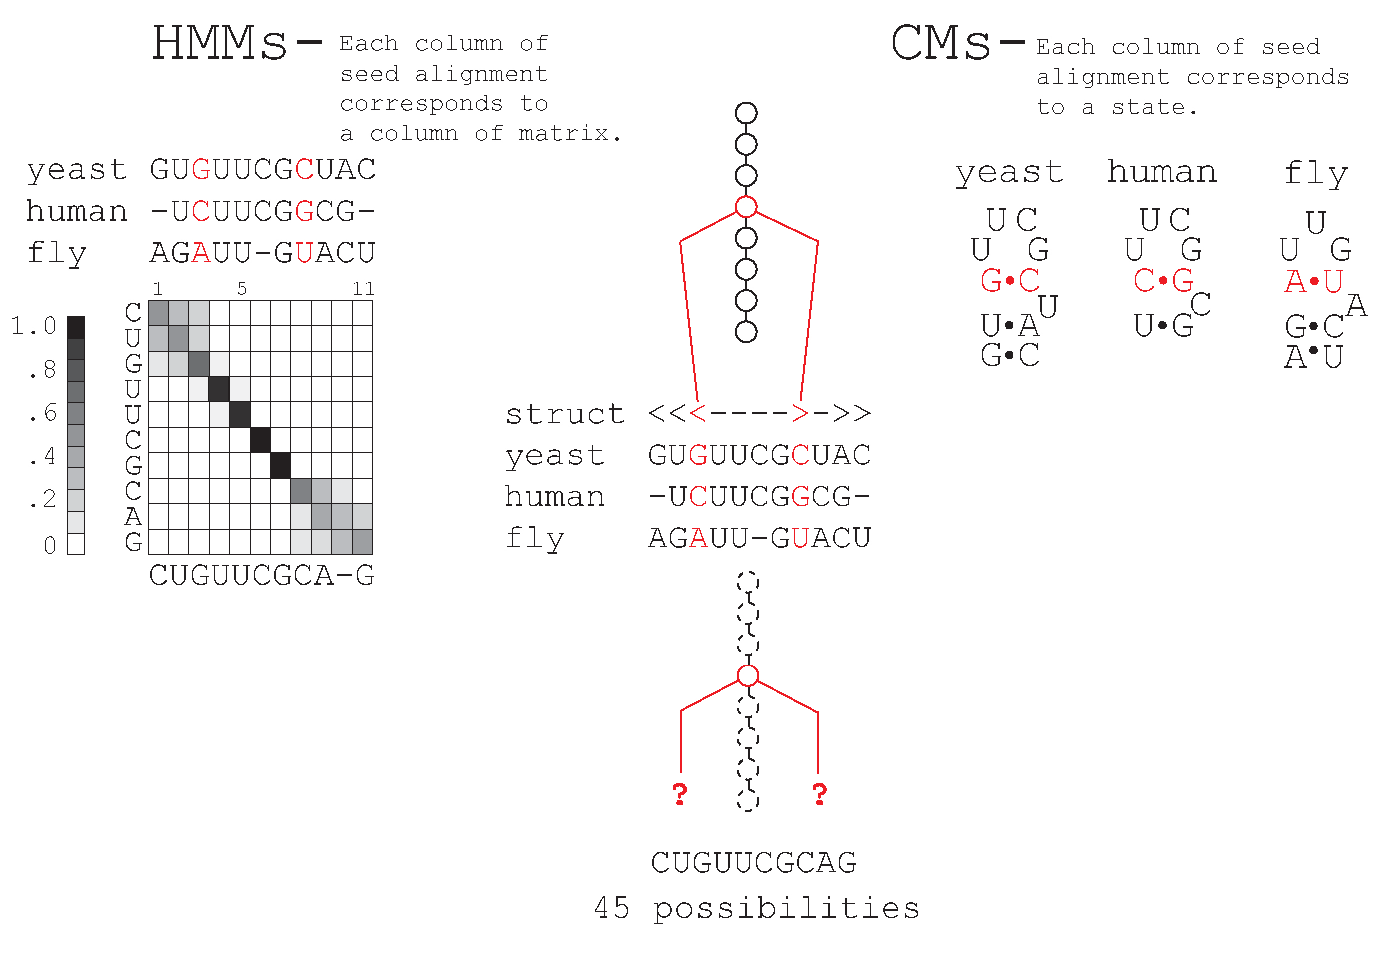
\includegraphics[width=8in]{figs/post_hmm_to_cm_map2_layer14}
\end{center}
\vfill
\end{slide}
%%%%%%%%%%%%%%%%%%%%%%%%%%%%%%%%%%%%%%%%%%%%%%%%%%%%%%%%%%%%%%%%%%%%%%%%%%
%%%%%%%%%%%%%%%%%%%%%%%%%%%%%%%%%%%%%%%%%%%%%%%%%%%%%%%%%%%%%%%%%%%%%%%%%%
\begin{slide}
\begin{center}

\textbf{HMM bands accelerate CM alignment}
\end{center}
\medskip
\small
\begin{itemize}
\item
\textbf{main idea:} eliminate potential alignments the HMM tells us are very improbable
\end{itemize}
\begin{center}
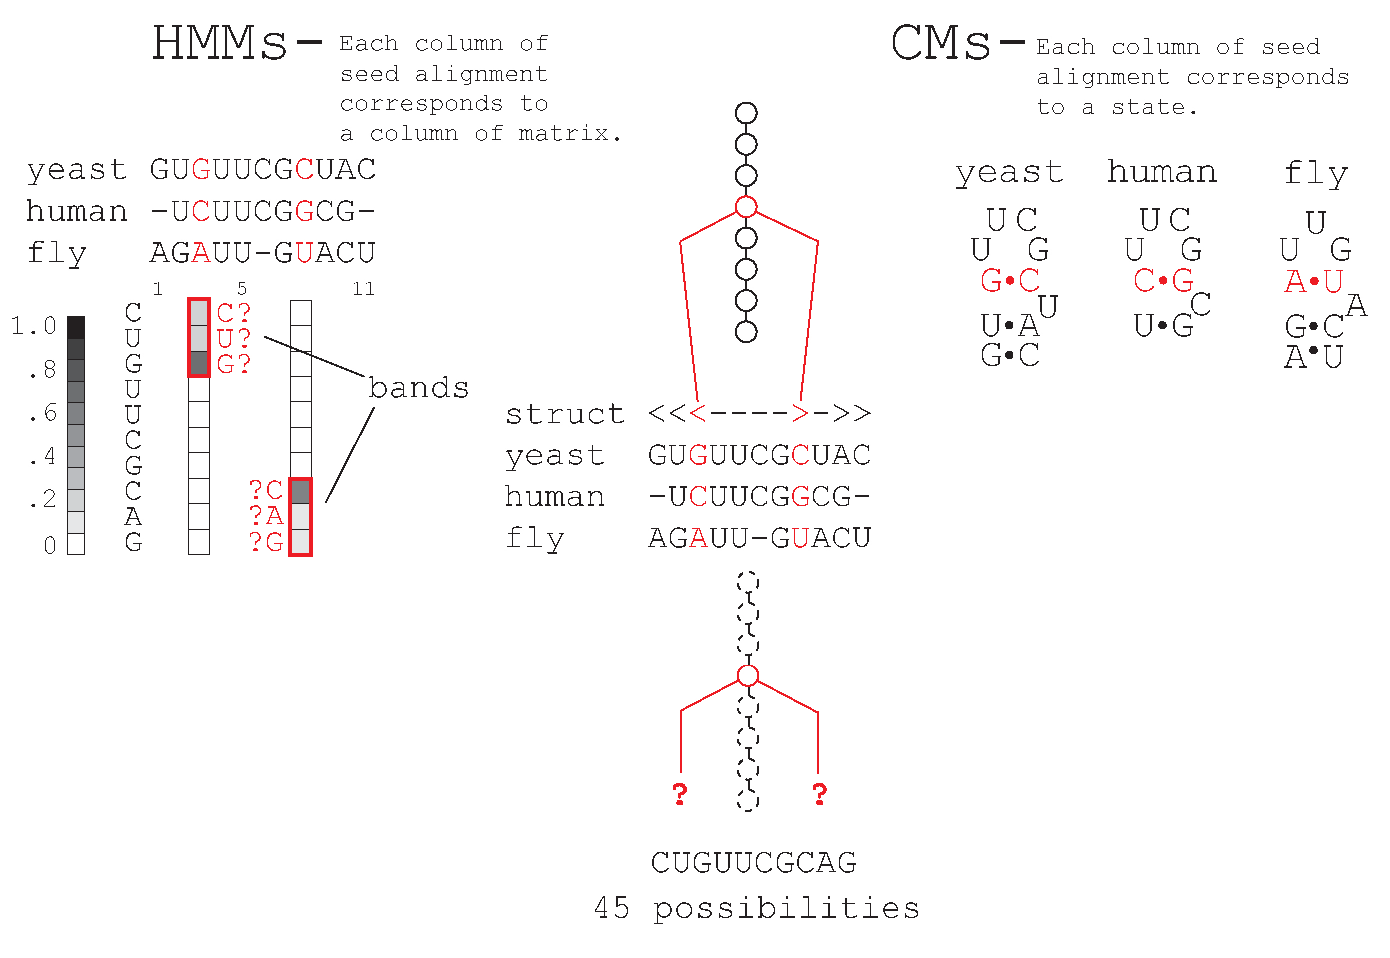
\includegraphics[width=8in]{figs/post_hmm_to_cm_map2_layer15}
\end{center}
\vfill
\end{slide}
%%%%%%%%%%%%%%%%%%%%%%%%%%%%%%%%%%%%%%%%%%%%%%%%%%%%%%%%%%%%%%%%%%%%%%%%%%
%%%%%%%%%%%%%%%%%%%%%%%%%%%%%%%%%%%%%%%%%%%%%%%%%%%%%%%%%%%%%%%%%%%%%%%%%%
\begin{slide}
\begin{center}

\textbf{HMM bands accelerate CM alignment}
\end{center}
\medskip
\small
\begin{itemize}
\item
\textbf{main idea:} eliminate potential alignments the HMM tells us are very improbable
\end{itemize}
\begin{center}
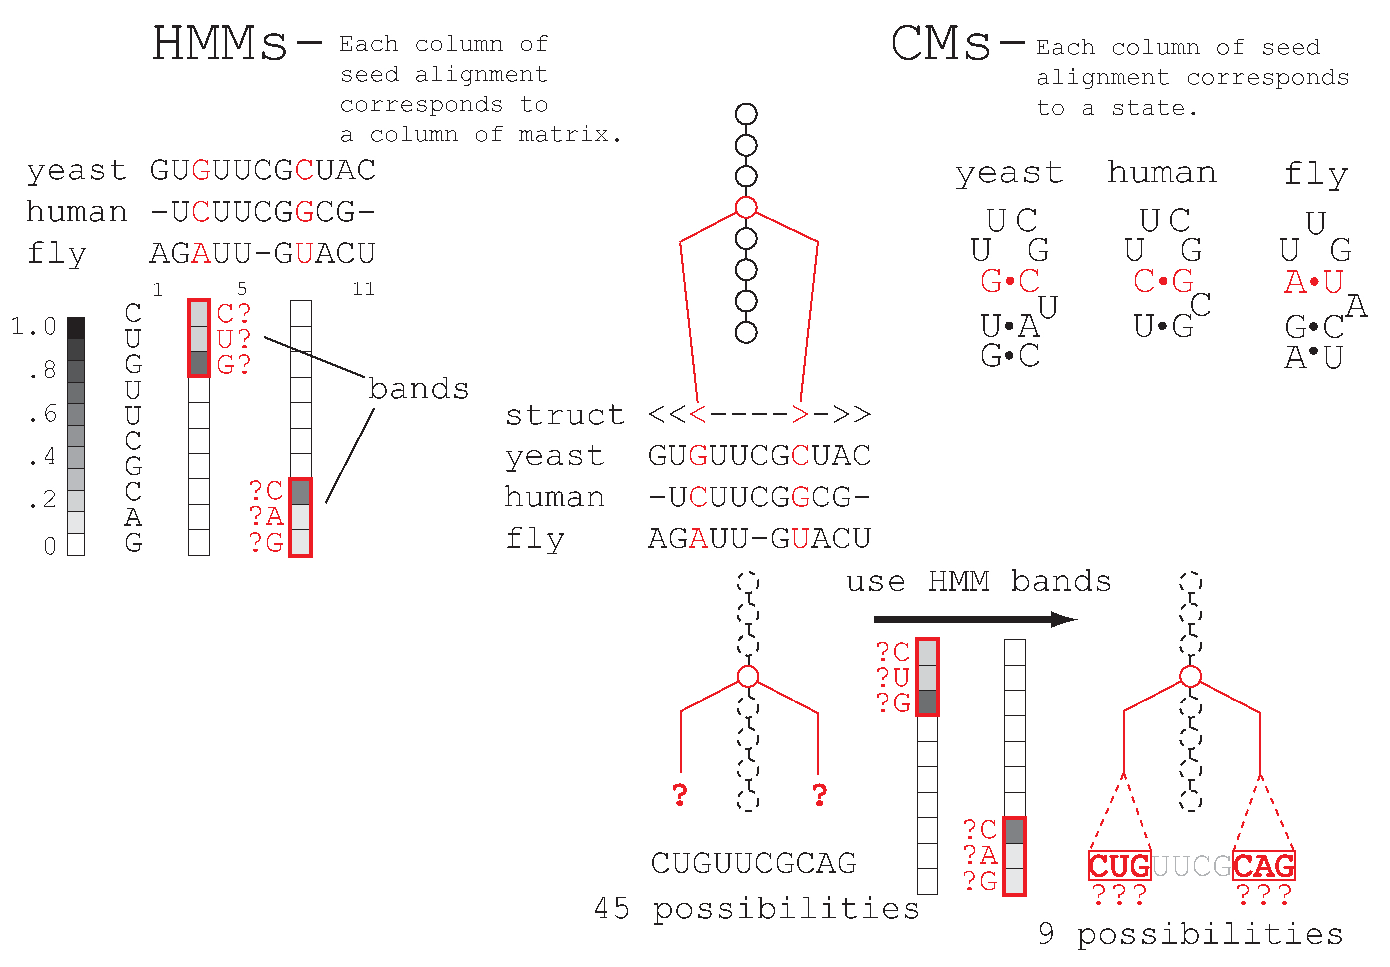
\includegraphics[width=8in]{figs/post_hmm_to_cm_map2_layer16}
\end{center}
\vfill
\end{slide}
%%%%%%%%%%%%%%%%%%%%%%%%%%%%%%%%%%%%%%%%%%%%%%%%%%%%%%%%%%%%%%%%%%%%%%%%%%

%%%%%%%%%%%%%%%%%%%%%%%%%%%%%%%%%%%%%%%%%%%%%%%%%%%%%%%%%%%%%%%%%%%%
\begin{slide}
\begin{center}
\textbf{Emission parameters using a mixture Dirichlet
  prior}\footnote{Durbin et al., \emph{Biological Sequence
      Analysis}, Oxford Univ Press, 1998.}
\end{center}
\medskip

\small

\begin{itemize}
\item probability of generating (emitting) residue $a$ from match state $j$: 

\begin{center}
$e_{M_j} (a) = \sum\limits_k P(k|\mathbf{c}_j) \frac{c_{ja} +
    \alpha_a^{k}}{\sum_{a'} (c_{ja'} + \alpha_a^{k})}$
\end{center}

\item where $\mathbf{c}_j$ are weighted counts of emissions 

\item where $p_k$ are the prior probabilities of the mixture components

\item and $P(k|\mathbf{c}_j)$ are the \emph{posterior mixture coefficients}:

\begin{center}
  $P(k|\mathbf{c}_j) = \frac{p_k P(\mathbf{c}_j|k)}{\sum_{k'}p_{k'}P(\mathbf{c}_j|k')}$
\end{center}

\item 
$P(\mathbf{c}_j|k)$ is the probability of the observed counts
($\mathbf{c}_j$) given the mixture component $k$:

\begin{center}

$P(\mathbf{c}_j|k) = \frac{(\sum_a c_{ja})!}{\prod_a c_{ja}!}
  \frac{\prod_a \Gamma(c_{ja} + \alpha_a^{k})}{\sum_a c_{ja}+\alpha_a^{k}}
  \frac{\Gamma(\sum_a \alpha_a^{k})}{\prod_a \Gamma(\alpha_a{^k})}$

\end{center}

\item Mixture components were estimated from large dataset of
alignment columns, by maximum likelihood (by minimizing the
log probability of $P(k|\mathbf{c}_j)$ given current parameters being
estimated via conjugate gradient descent)\footnote{Sjolander et al,
  Comput Appl Biosci 12: 327-345, 1996.}.

\end{itemize}

\vfill
\end{slide}
%%%%%%%%%%%%%%%%%%%%%%%%%%%%%%%%%%%%%%%%%%%%%%%%%%%%%%%%%%%%%%%%%%%%
\begin{slide}

\large
\begin{center}
\large{\textbf{Acknowledgements}} \\

\vspace{0.5in}

\normalsize
%\begin{tabular}{llllll}
%Sean Eddy           & & & & & Michael Brent \\ 
%Elena Rivas         & & & & & Jeremy Buhler \\
%Tom Jones           & & & & & Justin Fay \\
%Diana Kolbe         & & & & & Jeff Gordon \\
%Seolkyoung Jung     & & & & & Rob Mitra \\
%Sergi Castellano    & & & & & Gary Stormo \\
%Fred Davis          & & & & & \\
%Lee Henry           & & & & & \\
%Michael Farrar      & & & & & \\
%Travis Wheeler      & & & & & \\
\begin{tabular}{l}
Sean Eddy           \\
Elena Rivas         \\
Tom Jones           \\
Diana Kolbe         \\
Seolkyoung Jung     \\
Sergi Castellano    \\
Fred Davis          \\
Lee Henry           \\
Michael Farrar      \\
Travis Wheeler      \\
\end{tabular}

\includegraphics[height=2.75in]{figs/jfrc-banner1}

\end{center}

\vfill
\end{slide}
%%%%%%%%%%%%%%%%%%%%%%%%%%%%%%%%%%%%%%%%%%%%%%%%%%%%%%%%%%%%%%%
\end{document}

